%%% Hlavní soubor. Zde se definují základní parametry a odkazuje se na ostatní části. %%%

%% Verze pro jednostranný tisk:
% Okraje: levý 40mm, pravý 25mm, horní a dolní 25mm
% (ale pozor, LaTeX si sám přidává 1in)
\documentclass[12pt,a4paper]{report}
\setlength\textwidth{145mm}
\setlength\textheight{247mm}
\setlength\oddsidemargin{15mm}
\setlength\evensidemargin{15mm}
\setlength\topmargin{0mm}
\setlength\headsep{0mm}
\setlength\headheight{0mm}
% \openright zařídí, aby následující text začínal na pravé straně knihy
\let\openright=\clearpage

%% Pokud tiskneme oboustranně:
% \documentclass[12pt,a4paper,twoside,openright]{report}
% \setlength\textwidth{145mm}
% \setlength\textheight{247mm}
% \setlength\oddsidemargin{15mm}
% \setlength\evensidemargin{0mm}
% \setlength\topmargin{0mm}
% \setlength\headsep{0mm}
% \setlength\headheight{0mm}
% \let\openright=\cleardoublepage

%% Použité kódování znaků: obvykle latin2, cp1250 nebo utf8:
\usepackage[utf8]{inputenc}

%% Ostatní balíčky
\usepackage{graphicx}
\usepackage{amsthm}
\usepackage{pgfplots}
\usepackage{float}

%% PGF Number format
\pgfkeys{
  /pgf/number format/precision=3,
  /pgf/number format/fixed,
  /pgf/number format/fixed zerofill=true
}

%% Balíček hyperref, kterým jdou vyrábět klikací odkazy v PDF,
%% ale hlavně ho používáme k uložení metadat do PDF (včetně obsahu).
%% POZOR, nezapomeňte vyplnit jméno práce a autora.
\usepackage[ps2pdf,unicode]{hyperref}   % Musí být za všemi ostatními balíčky
\hypersetup{pdftitle=Modular Objective-C Run-Time Library}
\hypersetup{pdfauthor=Bc. Kryštof Váša}

%%% Drobné úpravy stylu

% Tato makra přesvědčují mírně ošklivým trikem LaTeX, aby hlavičky kapitol
% sázel příčetněji a nevynechával nad nimi spoustu místa. Směle ignorujte.
\makeatletter
\def\@makechapterhead#1{
  {\parindent \z@ \raggedright \normalfont
   \Huge\bfseries \thechapter. #1
   \par\nobreak
   \vskip 20\p@
}}
\def\@makeschapterhead#1{
  {\parindent \z@ \raggedright \normalfont
   \Huge\bfseries #1
   \par\nobreak
   \vskip 20\p@
}}
\makeatother

% Toto makro definuje kapitolu, která není očíslovaná, ale je uvedena v obsahu.
\def\chapwithtoc#1{
\chapter*{#1}
\addcontentsline{toc}{chapter}{#1}
}

\begin{document}

% Trochu volnější nastavení dělení slov, než je default.
\lefthyphenmin=2
\righthyphenmin=2

%%% Titulní strana práce

\pagestyle{empty}
\begin{center}

\large

Charles University in Prague

\medskip

Faculty of Mathematics and Physics

\vfill

{\bf\Large MASTER THESIS}

\vfill

\centerline{\mbox{\includegraphics[width=60mm]{img/logo.eps}}}

\vfill
\vspace{5mm}

{\LARGE Bc. Kry\u{s}tof V\'{a}\u{s}a}

\vspace{15mm}

% Název práce přesně podle zadání
{\LARGE\bfseries Modular Objective-C Run-Time Library}

\vfill

% Název katedry nebo ústavu, kde byla práce oficiálně zadána
% (dle Organizační struktury MFF UK)
Department of Distributed and Dependable Systems

\vfill

\begin{tabular}{rl}

Supervisor of the master thesis: & Mgr. Martin D\u{e}ck\'y \\
\noalign{\vspace{2mm}}
Study programme: & Informatics \\
\noalign{\vspace{2mm}}
Specialization: & Systémové architektury \\
\end{tabular}

\vfill

% Zde doplňte rok
Prague 2013

\end{center}

\newpage

%%% Následuje vevázaný list -- kopie podepsaného "Zadání diplomové práce".
%%% Toto zadání NENÍ součástí elektronické verze práce, nescanovat.

%%% Na tomto místě mohou být napsána případná poděkování (vedoucímu práce,
%%% konzultantovi, tomu, kdo zapůjčil software, literaturu apod.)

\openright

\noindent
My many thanks go to my supervisor Mgr. Martin D\u{e}ck\'y for his help with this thesis and to David Chisnall for replying to my questions about his run-time.

\newpage

%%% Strana s čestným prohlášením k diplomové práci

\vglue 0pt plus 1fill

\noindent
I declare that I carried out this master thesis independently, and only with the cited
sources, literature and other professional sources.

\medskip\noindent
I understand that my work relates to the rights and obligations under the Act No.
121/2000 Coll., the Copyright Act, as amended, in particular the fact that the Charles
University in Prague has the right to conclude a license agreement on the use of this
work as a school work pursuant to Section 60 paragraph 1 of the Copyright Act.

\vspace{10mm}

\hbox{\hbox to 0.5\hsize{%
In ........ date ............
\hss}\hbox to 0.5\hsize{%
signature of the author
\hss}}

\vspace{20mm}
\newpage

%%% Povinná informační strana diplomové práce

\vbox to 0.5\vsize{
\setlength\parindent{0mm}
\setlength\parskip{5mm}

Název práce:
Modular Objective-C Run-time Library
% přesně dle zadání

Autor:
Bc. Kry\u{s}tof V\'{a}\u{s}a

Katedra:  % Případně Ústav:
Department of Distributed and Dependable Systems
% dle Organizační struktury MFF UK

Vedoucí diplomové práce:
Mgr. Martin D\u{e}ck\'y, Department of Distributed and Dependable Systems
% dle Organizační struktury MFF UK, případně plný název pracoviště mimo MFF UK

Abstrakt:
This thesis contains analysis of currently available Objective-C run-time libraries (from GCC, Apple and \'Etoil\'e Runtime), their prerequisites, dependencies to particular platform and operating system as well as how components of the libraries depend on each other. The result of the analysis is a design of a modular run-time library that allows dynamic configuration of each component for particular need and platform (e.g. disabling structure locks in a single-thread environment, usage of custom data structures that are needed by the run-time). 

A prototype implementation of such a modular run-time for Objective-C also is included.

% abstrakt v rozsahu 80-200 slov; nejedná se však o opis zadání diplomové práce

Klíčová slova:
Objective-C, run-time
% 3 až 5 klíčových slov

\vss}\nobreak\vbox to 0.49\vsize{
\setlength\parindent{0mm}
\setlength\parskip{5mm}

Title:
Modular Objective-C Run-time Library

Author:
Bc. Kry\u{s}tof V\'{a}\u{s}a

Department:
Název katedry či ústavu, kde byla práce oficiálně zadána
% dle Organizační struktury MFF UK v angličtině

Supervisor:
Mgr. Martin D\u{e}ck\'y, Department of Distributed and Dependable Systems
% dle Organizační struktury MFF UK, případně plný název pracoviště
% mimo MFF UK v angličtině

Abstract:
This thesis contains analysis of currently available Objective-C run-time libraries (from GCC, Apple and \'Etoil\'e Runtime), their prerequisites, dependencies to particular platform and operating system as well as how components of the libraries depend on each other. The result of the analysis is a design of a modular run-time library that allows dynamic configuration of each component for particular need and platform (e.g. disabling structure locks in a single-thread environment, usage of custom data structures that are needed by the run-time). 

A prototype implementation of such a modular run-time for Objective-C also is included.
% abstrakt v rozsahu 80-200 slov v angličtině; nejedná se však o překlad
% zadání diplomové práce

Keywords:
Objective-C, run-time
% 3 až 5 klíčových slov v angličtině

\vss}

\newpage

%%% Strana s automaticky generovaným obsahem diplomové práce. U matematických
%%% prací je přípustné, aby seznam tabulek a zkratek, existují-li, byl umístěn
%%% na začátku práce, místo na jejím konci.

\openright
\pagestyle{plain}
\setcounter{page}{1}
\tableofcontents

\setcounter{secnumdepth}{3}

%%% Jednotlivé kapitoly práce jsou pro přehlednost uloženy v samostatných souborech
\chapter*{Introduction}
\addcontentsline{toc}{chapter}{Introduction}

While there already are existing Objective-C run-times, a closer look at them will show their weaknesses - mostly their dependencies or assumptions about the underlying OS and environment, where are they supposed to be running. Be it the POSIX layer, minimal object size, or GCC-specific C language extensions, all of these dependencies may present an obstacle when trying to compile such a run-time for a non-typical operating system (for example an experimental one), or when trying to use the Objective-C run-time in the kernel code.

This thesis will analyze source codes of existing versions of Objective-C run-time, their limitations or requirements for compilation. Result of this work will be a prototype of a modular Objective-C run-time, which will allow easy configuration of the run-time environment both at the compilation and run time. For example, for a single-threaded application, you will be able to turn off locking of internal structures without affecting stability, yet performance can be improved (with each message sent\footnote{In Objective-C method calls are called messages being sent to objects, just like in Smalltalk.}, a lock can be potentially locked when the method implementation isn't cached and the class hierarchy has to be searched) - this may save quite a few calls to the kernel.

There are three available Objective-C run-time implementations (to my knowledge) - one is provided by \emph{Apple} and is used in its OS X and iOS systems - there are slight differences between the iOS and OS X versions of the run-time (e.g.\ iOS doesn't support garbage collection and only the new 2.0 run-time is available). Within this thesis, when talking about Apple's implementation of the run-time, the OS X version will be the one talked about. Then there's a run-time provided with \emph{GCC} compiler and a more experimental one called \emph{\'{E}toil\'{e}} which has been used to improve the \emph{GNUStep} run-time\footnote{http://www.jot.fm/issues/issue\_2009\_01/article4/index.html}.

Even though I will mention a few words about the garbage collection and ARC\footnote{ARC - automatic reference counting, a feature introduced in Xcode 4.2 (Xcode is Apple's IDE) that uses compiler's static analysis combined with special keywords to automatically insert retain/release calls so that the developer doesn't need to manually manage reference counts on objects.}, not much attention will be paid to them as garbage collection is being deprecated in OS X 10.8 (and has severe dependencies on the underlying operating system itself) and ARC is a relatively new technology which uses a lot of compiler-dependent features as well as auto-zeroing weak references, etc.; which is beyond the scope of this work. Instead, the focus will be put on the core functionality of the run-time, analysis of the current implementations and designing the modular run-time itself.
\chapter{What Is a Run-Time?}

With every object-oriented language a question arises - what makes an object object - how is it represented in the memory. In its core it is a structured piece of memory that could be representable by a structure in the C language. In particular, an object in Objective-C is defined as a structure, whose first field is a so-called \verb=isa= pointer, pointing to the object's class.

With this in mind, a new question pops up - what are methods and how are the method calls performed?

In languages, such as C, it is already known which code should be executed when you call a particular function. The linker then links function calls directly to the address the function resides at. 

Imagine an object-oriented language, where each class had a compile-time known number of methods, these methods could be a part of the class structure, so each method call would consist of just reaching for the correct function pointer within the object's class structure.

This gets more complicated once we take class hierarchy into consideration. Each class can override methods of its parent class, which can be solved by using the same function 'slot'.

Let us demonstrate this on an example written in pseudo-code:

\begin{figure}[H]
  \begin{verbatim}
/** Memory representation of an object. */
struct object_structure {
  class_structure_t *class;
  
  /** Other fields follow. */
} object_structure_t;

/** Memory representation of a class. */
struct class_structure {
  struct class *super_class;
  
  /** Function array of unknown size */
  void*(**functions)(object_structure_t *, ...);
} class_structure_t;
  \end{verbatim}
  \centering{}
  \caption{Structures representing an object and a class.}
  \label{fig:imaginary_lang_structs}
\end{figure}


\begin{figure}[H]
  \begin{verbatim}
class Class1 {
  void method1();
  int method2();
}

class Class2 extends Class1 {
  override void method1();
}
  \end{verbatim}
  \centering{}
  \caption{Declaring two classes.}
  \label{fig:imaginary_lang_classes}
\end{figure}

In this example, \verb=method1= of \verb=Class1= would reside in \verb=Class1->functions[0]=, \verb=method2= in \verb=Class2->functions[1]=, \verb=method1= of \verb=Class2= would reside in \newline{}\verb=Class2->functions[0]=. Hence if \verb=my_obj.method1()= were to be called, it could get translated into \verb=my_obj->class->functions[0]()=.

This, however, brings up a few issues:

\begin{itemize}
  \item{\bf{Binary compatibility}} Linking against a framework which has \verb=method1= in \verb=functions[0]= does not mean the next version will do too - it is the compiler that would decide the order of the functions in the \verb=functions= field.
  \item{\bf{No duck-typing}} If \verb=Class2= is not a subclass of \verb=Class1=, yet implements a method with the same signature - name, types - this would not work either.
  \item{\bf{Extending classes at run time}} All methods must be known at compile time. No methods may be added using e.g. categories like in Objective-C.
\end{itemize}

The solution to these issues is to move to a dynamic dispatch - a mechanism that finds the correct method implementation for that particular object. In this example case, instead of the \verb=functions= field on the class structure, there would be a \verb=methods= field. This methods field would contain a list of methods and the dispatch would look at the name of the method to be invoked, look up the correct implementation and call it. It must be obvious that such a mechanism has its performance cost as calling methods on objects is one of the most common tasks in object-oriented programming.

The \emph{run-time}, being responsible for this dispatch among other tasks, must hence perform this look-up as fast as possible. Other responsibilities of the run-time are to provide a reflection API to constructs of that particular language. For example, listing classes and their methods, exchanging method implementations, listing ivars, etc.


\section{Existing Objective-C Run-Time Implementations}

There are three available Objective-C run-time implementations (to my knowledge):

\begin{itemize}
  \item{\bf{Apple Run-Time}} This run-time is provided by \emph{Apple} and is used in its OS X and iOS systems - there are slight differences between the iOS and OS X versions of the run-time (e.g.\ iOS doesn't support garbage collection and only the new 2.0 run-time is available). Within this thesis, when talking about Apple's implementation of the run-time, the OS X version will be the one talked about.
  \item{\bf{GCC Run-Time}} Also called GNU, or GNUstep run-time, this run-time is provided with the GCC compiler. The naming is a little confusing - the run-time is bundled with the GCC compiler, yet is often referred to as GNU run-time. In 2009, a fork of the run-time's repository has been created to add the newest run-time features and remove legacy code. This fork is called GNUstep run-time. Because both run-times are similar in many ways, both run-times are referred to as the GCC run-time within this thesis.
  \item{\bf{\'{E}toil\'{e}}} \'{E}toil\'{e} is an experimental run-time written by David Chisnall as a part of his paper and has been an inspiration to many improvements in the GNUstep run-time\footnote{http://www.jot.fm/issues/issue\_2009\_01/article4/index.html}.
\end{itemize}


\chapter{Objective-C}
  
In the early 1980s, Brad Cox and Tom Love decided to bring the object-oriented concept to the world of C while maintaining full backward compatibility. The result was Objective-C, a language heavily inspired by Smalltalk. At first, the language had no compiler support, but as all Objective-C code can be actually rewritten in pure C, a preprocessor was a sufficient tool.

In 1988, NeXT has licensed Objective-C from Stepstone (the company Cox and Love owned), added Objective-C support to the GCC compiler and decided to use it in its OpenStep and NeXTSTEP operating systems (many classes in Apple's frameworks have a \verb=NS= prefix to the date, which stands either for NeXTSTEP, or NeXT-Sun as the OpenStep operating system had been developed in cooperation with Sun Microsystems\footnote{http://en.wikipedia.org/wiki/OpenStep}).

After Apple had acquired NeXT in 1996, Objective-C stayed alive in Rhapsody\footnote{http://en.wikipedia.org/wiki/Rhapsody\_(operating\_system)} and later on in Mac OS X, where it is the preferred programming language to the date.

For this whole time, the Objective-C language stayed almost the same without any significant changes, until 2006, when Apple announced Objective-C 2.0 (released as a part of Mac OS X 10.5 in 2007), which introduced garbage collection (since then deprecated in 10.8 in favor of more efficient ARC - automatic reference counting\footnote{http://cocoaheads.tumblr.com/post/17719985728/10-8-objective-c-enhancements}), properties (object variables with automatically generated getters and/or setters with specified memory management), fast enumeration (enumeration over collections in a foreach-style), and some other minor improvements.

Lately, more improvements have been made to Objective-C, most importantly the aforementioned ARC (automatic reference counting). Apple's run-time has a hardcoded set of selectors (method names) that handle the memory management, \verb=-autorelease=, \verb=-retain=, \verb=-release= (together called ARR), in particular. ARC automatically inserts these method calls and automatically generates a \verb=-dealloc= method (which is called when the object is being deallocated) - this, however, adds a heavy dependency on the compiler, though, as it needs to statically analyze the code in order to safely insert these ARR calls.

This, however, presents a problem - none of the ARR calls must be called directly in the code - hence all code needs to be converted to ARC\@. One disadvantage which results in a big advantage - compatibility with all existing frameworks. The backward incompatibility was a big disadvantage of garbage collection: 

The code could be kept as it was - the run-time itself redirects the ARR methods to a no-op function on the fly. All linked libraries / frameworks / plugins, however, needed to be recompiled with garbage collection support turned on. This caused two things: mess in the code as the code migrated to garbage-collection-enabled environment was riddled with ARR calls, but newly written code typically missed those calls, making the code inconsistent. Also, some libraries never got GC support anyway, so they couldn't be used in GC-enabled applications.

In the newest release of OS X - 10.8, several more new features have been included - default synthesis of getters (in prior versions, you had to declare \verb=@property= in the header file and use \verb=@sythesize= or \verb=@dynamic= in the implementation file), type-safe enums, literals for \verb=NSArray=, \verb=NSDictionary= and \verb=NSNumber= (classes declared in Apple's Foundation framework), etc.

\section{Objective-C Syntax in a Nutshell}

While a complete reference to the language is not a goal of this work, a quick syntax overview is included for readers without any Objective-C knowledge.

\subsection{Class Declaration}

A class can be declared using the following notation:

\begin{figure}[H]
  \begin{verbatim}
@interface Class : Superclass {
  int anIvar;
}

// Method and property declarations follow:

+(void)classMethod;

-(int)instanceMethod;

@property BOOL myProperty;

@end
  \end{verbatim}
  \centering{}
  \caption{Declaration of an Objective-C class.}
  \label{fig:syntax_objc_class_decl}
\end{figure}

The class declaration may be divided into two sections:

\begin{itemize}
  \item{\bf{Ivars}} A list of ivars, which can be completely omitted if the class has no ivars to declare.
  \item{\bf{Method and property declarations}} Methods and properties may be declared here. Methods that start with the \verb=+= sign are class (static) methods, methods starting with the \verb=-= sign are instance methods.
\end{itemize}

After declaring a class, it needs to be implemented as well:

\begin{figure}[H]
  \begin{verbatim}
@implementation Class

+(void)classMethod{
  // Method body goes here
}

-(int)instanceMethod{
  // Method body goes here
}

@end
  \end{verbatim}
  \centering{}
  \caption{Implementation of an Objective-C class.}
  \label{fig:syntax_objc_class_impl}
\end{figure}

In earlier versions of the run-time (and OS), each property had to be matched with a \verb=@synthesize= construct in the implementation part of the class, which is no longer necessary as it gets generated automatically.

\subsection{Declaring Methods}

As has been seen in figure ~\ref{fig:syntax_objc_class_decl}, each method declaration begins with either a \verb=+= sign (class method), or \verb=-= sign (instance method), followed by a return type, method name and potentially arguments.

If the method should have an argument, it is followed by a semicolon, type of the argument and the argument name:

\begin{figure}[H]
  \begin{verbatim}
-(void)setName:(NSString*)name;
  \end{verbatim}
  \centering{}
  \caption{Method declaration with a single argument.}
  \label{fig:syntax_objc_single_arg}
\end{figure}

More arguments are allowed as well, splitting the method name:

\begin{figure}[H]
  \begin{verbatim}
-(void)writeToFileAtURL:(NSURL*)url 
              usingEncoding:(NSStringEncoding)enc;
  \end{verbatim}
  \centering{}
  \caption{Method declaration with multiple arguments.}
  \label{fig:syntax_objc_multiple_args}
\end{figure}

\subsection{Calling Methods}

Calling methods, or in Smalltalk's terminology sending messages, is achieved using the following formulations:

\begin{figure}[H]
  \begin{verbatim}
[Class classMethod];
[obj instanceMethod];
[obj setName:@"John"];
[obj writeToFileAtURL:url usingEncoding:NSUTF8StringEncoding];
  \end{verbatim}
  \centering{}
  \caption{Calling methods on a class and an object.}
  \label{fig:syntax_objc_msg_sending}
\end{figure}

\subsection{Miscellaneous}

\begin{itemize}
  \item{\bf{Strings}} As regular C strings cannot be treated as an object, a special notation is introduced for Objective-C strings - \verb=@"String"=.
  \item{\bf{Synchronization}} A special synchronization construct \newline{}\verb=@synchronized(obj){ ... }= can be used for critical section code.
  \item{\bf{Hidden variables}} In each method, three special variables may be accessed: \verb=self= (pointing to the object itself), \verb=_cmd= (the method name) and \verb=super= (allowing invocation of the superclass' implementation of methods).
\end{itemize}


\section{Compilation of Objective-C}

Objective-C is an object-oriented programming language that is a strict superset of C. Any C code can be used within Objective-C source code. Its run-time is written in C as well, some parts in the assembly language (mostly performance optimizations) or more recently in C++ (more about that later on).

And the other way around, all Objective-C code can be translated to calls of C run-time functions. There is an LLVM Clang compiler option \verb=-rewrite-objc= which converts all the Objective-C syntax into calls of pure C methods - the run-time methods. When run 

\begin{verbatim}
  clang -rewrite-objc test.m
\end{verbatim}

where \verb=test.m= contains the Objective-C code, a new test.cpp is created, containing the translated code. For example, sending a message to an object is nothing else but calling a run-time function \verb=objc_msgSend=. Note that the run-time implementations may differ in the function names, or even use different structures and the way methods are invoked. The examples below will show how the code translation works with Apple's version of the run-time. These examples are here to simply illustrate the mechanism of translating Objective-C code to C constructs.

\subsection{Calling methods}

As has been mentioned before, calling a method is not anything else than calling a \verb=objc_msgSend= variadic function, which is responsible for finding a function pointer that implements the actual method and invoking it, passing all the arguments along

\paragraph{Example}
Here is a sample code that sends two messages - each to a different object, though - each class actually consists of two classes - the meta class, which implements the \verb=+alloc= method and the regular class (an instance of the metaclass), which implements the \verb=-init= method.

\begin{verbatim}SomeClass *myObj = [[SomeClass alloc] init];\end{verbatim}

This gets to be translated to:
\begin{verbatim}SomeClass *myObj = ((id (*)(id, SEL, ...))(void *)objc_msgSend)
              ((id)((id (*)(id, SEL, ...))(void *)objc_msgSend)
                                  (objc_getClass("SomeClass"),
                                  sel_registerName("alloc")), 
                                  sel_registerName("init"));
\end{verbatim}

Which after removing the casting and adding a little formatting is equivalent with:

\begin{figure}[H]
  \begin{verbatim}SomeClass *myObj = 
  objc_msgSend(
    objc_msgSend(
      objc_getClass("SomeClass"),  
      sel_registerName("alloc")), 
    sel_registerName("init"));
  \end{verbatim}
  \centering{}
  \caption{Objective-C message calls translated to run-time function calls.}
  \label{fig:methods_translated_to_objcMsgSend}
\end{figure}

So it is two nested \verb=objc_msgSend= calls. There are actually specific functions for methods that return floating point numbers or structures, as these require special ABI treatment on some architectures - for example structures that do not fit into registers are returned by reference on the stack as a hidden first argument of the function. \verb=objc_msgSend= is a function that can be called the core of Objective-C run-time. It is the most used function of the run-time. Every method call in Objective-C gets translated into this variadic function call, which takes \verb=self= as the first argument (i.e.\ the object the message is sent to), the second argument is a selector (generally the method's name) and can be followed by any number arguments.

\subparagraph{GCC Run-time}

The GCC run-time differs slightly from Apple's run-time - it does not have a \verb=objc_msgSend= function, but uses \verb=objc_msg_lookup= function, which rather returns a pointer to the implementation function itself (the so-called \verb=IMP=). The same example would compile under the GCC run-time into the following calls:

\begin{figure}[H]
\begin{verbatim}
  id receiver1 = objc_getClass("SomeClass");
  SEL selector1 = sel_registerName("alloc");
  IMP allocIMP = objc_msg_lookup(receiver1, 
                                  selector1);
  id receiver2 = allocIMP(receiver1, selector1);
  SEL selector2 = sel_registerName("init");
  IMP initIMP = objc_msg_lookup(receiver2, 
                                  selector2);
  SomeClass *myObj = initIMP(receiver2, selector2);
\end{verbatim}
\centering{}
  \caption{Objective-C message calls translated to run-time function calls in GCC run-time.}
  \label{fig:methods_translated_to_objc_msg_lookup}
\end{figure}

As you can see, Apple's run-time differs only in the fact that the \verb=objc_msgSend= calls the function directly, whereas the GCC run-time looks up the function and then calls it. This has a small advantage that it does not require any special variants of functions, like in Apple's run-time, where the \verb=objc_msgSend= has 4 variants depending on the return type.

\hspace{20pt}

But even so, the principe is the same as in Apple's run-time. The run-time needs to look up the object's class, find a function that implements that particular method (the so called \verb=IMP=) and the function gets called either by \verb=objc_msgSend=, or directly. There are several things to point out:

\begin{itemize}
\item method \emph{names} are used. \verb=sel_registerName= is a function that makes sure that for that particular method name only one selector pointer is kept. A selector is a pointer to a structure representing a method name. On some run-times, selectors are typed, i.e.\ methods of the same name, but with different argument types result in different selectors. While Objective-C does not support method overloading, the selector storage is program-wise, not just per class.
\item every class consists of two classes - a class pair - one regular of which you create objects and one meta - which typically (unless you manually craft another one) has only one instance: a receiver for class methods (static methods).
\item each of the calls is sent to a different object. The first call is sent to something returned by \verb=objc_getClass= which returns a class, which is an instance of its meta class (which is an object as well). The second call goes already to an object - instance of the class (the class hierarchy is described below).
\end{itemize}

\paragraph{Calls to super}

Objective-C, as most object-oriented languages, allows calls of the method implementations of a superclass using the keyword \verb=super=. For example, the \verb=-init= method usually starts with \verb#if ((self = [super init]) != nil)#. This is done using a special structure \verb=objc_super=, which is passed by reference to \verb=objc_msgSendSuper= (or its relatives) in case of Apple run-time, or \newline{}\verb=objc_msg_lookup_super= in case of GCC run-time.

\subparagraph{Example}

\begin{verbatim}
-(void)someMethod:(void*)firstArgument{
  [super someMethod:firstArgument];
}
\end{verbatim}

Is equivalent to:

\begin{figure}[H]
\begin{verbatim}
-(void)someMethod:(void*)firstArgument{
  struct objc_super super = { 
      self, 
      class_getSuperclass(objc_getClass("SomeSubclass")) 
  };
  objc_msgSendSuper(&super, 
                    sel_registerName("someMethod:"), 
                    firstArgument);
}
\end{verbatim}
\centering{}
  \caption{Objective-C message call to super translated to a run-time function call.}
  \label{fig:methods_translated_to_objcMsgSendSuper}
\end{figure}

\subsection{Object Model}

As Objective-C is heavily influenced by Smalltalk, let us examine the Smalltalk object model first\footnote{All copyright for this image goes to Andrew P. Black St\'{e}phane Ducasse, Oscar Nierstrasz Damien Pollet and Damien Cassou and Marcus Denker - http://pharo.gforge.inria.fr/PBE1/PBE1.html}:

\begin{figure}[H]
\includegraphics[width=120mm]{./img/smalltalk_class_hierarchy.png}
  \centering{}
  \caption{Smalltalk's object model.}
  \label{fig:smalltalk_obj_model}
\end{figure}

The model may seem complex and even a little confusing in some areas. Smalltalk's approach that everything is an instance of some class poses a question where is the end to the class hierarchy? Most languages that introduce a concept of a metaclass have to solve this by a loop: in Smalltalk's case, it is the loop between \verb=Metaclass= and \verb=Metaclass class=, where each is an instance of the other. The Objective-C object model indeed has a similar loop, however. It is not that complex and would end at the \verb=Object class= point in the Smalltalk diagram.

\paragraph{Root Class}
The \verb=NSObject= class is part of the Foundation framework Apple supplies. While it is often assumed to be the one and only root class in Objective-C, this is quite incorrect: there can be as many root classes in Objective-C as you wish - \verb=NSProxy= is an example and you can easily create your own:

\begin{figure}[H]
\begin{verbatim}@interface ClassWithoutSuperclass {
  
}

@end\end{verbatim}
  \centering{}
  \caption{Declaring a root class in Objective-C.}
  \label{fig:objc_root_class}
\end{figure}

This declares a new root class. It has absolutely no functionality - no memory management methods such as \verb=-retain= and \verb=-release=, no \verb=+alloc= method is declared either - it is impossible to even create a new instance of this class without the run-time function \verb=class_createInstance= - which is basically why it is recommended to inherit all classes from NSObject (or any other already prepared root class) which implements some basic communication with the run-time as well as some basic memory management, etc. Also, Apple's run-time has hardcoded references to \verb=NSObject=, which enables faster ARR message dispatch (as it checks if the class has any custom ARR-method implementation).

In Objective-C, each object is a pointer to a structure, where the first member is a so-called \verb=isa= pointer. Actually, the \verb=id= type, that represents any Objective-C object is defined as follows:

\begin{figure}[H]
\begin{verbatim}
typedef struct objc_class *Class;
typedef struct {
  Class isa;
} *id;
\end{verbatim}
  \centering{}
  \caption{Objective-C's object definition.}
  \label{fig:objc_obj_def}
\end{figure}

To support the behavior that a class (\verb=Class=) is an object as well, the class structure begins with the \verb=isa= pointer, which points to its meta class. The \verb=isa= pointer is followed by a \verb=superclass= field and many others - ivars, methods, cache, dispatch table, etc. - depending also on the run-time that you are using - you should hence never rely on the class structure itself, it should be treated as an opaque structure, with the internals exposed only to the run-time itself. To simplify this example, let us use this simplified class structure:

\begin{figure}[H]
\begin{verbatim}
typedef struct class_t {
  struct class_t *isa;
  struct class_t *superclass;
  
  // Actually, more fields follow
} objc_class_t;
\end{verbatim}
  \centering{}
  \caption{Simplified structure representing an Objective-C class.}
  \label{fig:objc_class_struct_simplified}
\end{figure}

For a regular class, the \verb=isa= pointer points to its meta class and the \verb=superclass= pointer points to its regular superclass, or \verb=Nil= in case it is the root class (in Objective-C, the zero pointer is called \verb=nil= for objects and \verb=Nil= for classes - both are just \verb=#define=s of a typed zero, though). 

Now how about the meta class? In case the class is not a root class, the \verb=superclass= pointer points to its meta superclass and the \verb=isa= pointer points to the same meta class.

Hence the regular class is an instance of its superclass. In case the class is a root class, its \verb=isa= pointer points to the structure itself, and its superclass is the regular class. Let's examine this on an example:

\begin{verbatim}@interface Rootclass{
  
}

@end

@implementation Rootclass

// Empty implementation

@end



@interface Subclass : Rootclass{

}

@end

@implementation Subclass

// Empty implementation

@end 
\end{verbatim}

This declares two classes (actually four, as for each class a meta class is created as well) - \verb=Rootclass= and \verb=Subclass=. The \verb=Rootclass= is a new root class with no superclass. As neither of these classes declares any methods, calling anything on either class would result in a run-time exception, even the usual object creation via \verb=[[Rootclass alloc] init]= is not available as \verb=Rootclass= does not declare the \verb=+alloc= method - it is declared on the \verb=NSObject= class, which is why you can create instances of the ``regular" classes inheriting from \verb=NSObject= this way.

Hence the run-time function \verb=class_createInstance= needs to be called in order to create an instance of the class:

\begin{verbatim}
id obj = class_createInstance(objc_getClass("Subclass"), 0);
\end{verbatim}

The \verb=objc_getClass= function returns a pointer to the class called \verb=Subclass=, the \verb=class_createInstance= function creates an instance of the \verb=Subclass= class, with \verb=0= extra bytes - the extra bytes parameter is here in case you wanted to dynamically add extra space to some of your instances, or to all by overriding the \verb=+alloc= method of the class. It is noteworthy that the \verb=+alloc= method is actually nothing else than \verb=-alloc= on the meta class - i.e.\ all class methods are in fact instance methods on the meta class.


Diagram on figure ~\ref{fig:class_metaclass_graph} visualizes this situation of two classes - one root class and its subclass; and an instance of the subclass.

\begin{figure}[H] 
\includegraphics[width=\textwidth]{img/metaclass_graph.png}
  \centering{}
  \caption{A graph of the class - meta-class relationship.}
  \label{fig:class_metaclass_graph}
\end{figure}

It is obvious from the diagram that the Objective-C object model is far less complicated than Smalltalk's. The class hierarchy ends at the point of the root class. To sum it up:

\begin{itemize}
\item Each class consists actually of two classes: the regular class and the meta class.
\item As the class hierarchy goes, the meta class hierarchy follows the regular class hierarchy up to the root class.
\item It is easy to detect a meta class - \verb:cl->superclass == cl->isa:.
\item Since the regular class is just an instance of the meta class, having a pointer to the meta class, there is no way of retrieving a pointer to the regular class. This is why the run-times store pointers to the regular classes and not their meta classes.
\item The root class is a little special, as the meta class is an instance of itself and its superclass is the regular class (which is an instance of the meta class).
\item This has a peculiar consequence: all instance methods of the root class are class methods as well. In the lookup chain, when the search on meta classes yields nothing, the run-time follows the \verb=superclass= pointer, which points to the regular class object. This can be easily verified:
\end{itemize}

\begin{figure}[H]
\begin{verbatim}
unsigned int number_of_methods = 0;
Method *methods, *method_ptr;
methods = method_ptr = class_copyMethodList([NSObject class], 
                                            &number_of_methods);
while (number_of_methods){
  printf("%s\n", sel_getName(method_getName(*methods)));
  ++methods;
  --number_of_methods;
}
free(method_ptr);
\end{verbatim}
  \centering{}
  \caption{Listing methods of \texttt{NSObject} class.}
  \label{fig:listing_NSObject_methods}
\end{figure}

This piece of code prints all available methods on a class. The \verb=[NSObject= \verb=class]=, however, is the regular class, which on the installation of OS X it has been tested, prints out 298 methods. Note that these are methods directly implemented by that class. Methods implemented by the class' superclasses are not included.

When \verb=[NSObject class]= is replaced with

\begin{verbatim}
methods = method_ptr = class_copyMethodList(
                                ((id)[NSObject class])->isa, 
                                &number_of_methods
                                           );
\end{verbatim}

a list of methods declared directly on the meta class is printed. This list counts only 118 methods, among which, for example, is not a method \verb=isNSArray__=, which is a private \verb=NSObject= instance method for deciding whether the object is an instance of \verb=NSArray= class. While the meta class itself does not implement this method, however, calling

\begin{verbatim}
[((id)[NSObject class])->isa isNSArray__];
\end{verbatim}

does not yield in any run-time exception, or similar, it simply invokes the instance method. This can be further proved by exchanging the function pointer of \verb=NSObject='s \verb=isNSArray__= method with a custom function, that prints a message, for example.

While this trickery might be viewed as unnecessary and almost 'insane', it has a good reasoning behind - it is mostly because of this that you can treat classes as regular objects without implementing the same methods twice - once as instance methods and once as class methods.

\subsection{Creating Classes Programmatically}

While this is not a feature of the run-time that would be used on a daily basis, classes can be created and inserted into the run-time at any time. There is a function called \verb=objc_allocateClassPair= which creates a brand new class and its meta class counterpart - together a class pair. All that is needed to be specified is the superclass, the new class' name and extra bytes. These extra bytes are similar to the extra bytes argument of \verb=objc_createInstance=, but this time they represent extra bytes on the class structure itself for possible class functionality extension. Run-time functions such as \verb=class_addMethod=, \verb=class_addIvar=, \verb=class_addProtocol= and \verb=class_addProperty= can be used to add methods, ivars, protocols and properties to a class.

Creating the class using the \verb=objc_allocateClassPair= function is not enough in order to create an instance of this class, though. It is necessary to register the class pair with the run-time as well, using \verb=objc_registerClassPair=. This is simply to avoid creating an instance of the class before it gets fully initialized, e.g.\ from a different thread. Using these functions, the Objective-C compiler may easily be substituted, creating all classes at the beginning of the program execution programatically.

In reality, declaring a class does not cause the compiler to generate function calls. Instead, the compiler creates static class structures which are later on copied by the linker into the \verb=__OBJC= section of the Mach-O binary (on OS X), which is copied on the launch time to memory and the classes just get registered with the run-time (the dynamic loader calls some private run-time methods for copying classes from binary images), which is much faster than dynamically creating classes one by one, connecting all methods, ivars, etc. This thesis, however, focuses on the run-time methods, ignoring linker and dynamic loader dependencies.

\subsection{Translating Methods to Functions}

As noted several times before, all Objective-C code can be rewritten in pure C code. This brings us to a question, how the methods are translated to C constructs - obviously into functions, so-called \verb=IMP=s (an implementation pointer). Let us use this class to demonstrate:

\begin{verbatim}

@implementation SomeClass
+(void)doSomethingStatic{
  // ...
}
-(void)someMethod:(void*)arg1 secondArgument:(void*)arg2{
  // ...
}
@end

\end{verbatim}

This gets translated into two functions:

\begin{figure}[H]
\begin{verbatim}
typedef struct objc_object SomeClass;

void _C_SomeClass_doSomethingStatic(Class self, SEL _cmd){
  // ...
}

void _I_SomeClass_someMethod_secondArgument(SomeClass *self,
                             SEL _cmd, void *arg1, void *arg2){
  //...
}
\end{verbatim}
  \centering{}
  \caption{Methods translated into C functions.}
  \label{fig:methods_translated_into_C_fncts}
\end{figure}

As can be seen, each method gets translated into a function of at least two arguments. The first argument is \verb=self= - a pointer to the object the message is being sent to. In the first case a \verb=Class= object, in the second case a pointer to the \verb=SomeClass= object. The second argument, \verb=_cmd=, is the selector (\verb=SEL=). Using a function with the same signature, method implementations of existing methods may be easily exchanged.

The function names get slightly obfuscated - \verb=_X_ClassName_method_name_= - where \verb=X= is either \verb=I= for instance methods or \verb=C= for class methods. As Objective-C method names can have multiple parts, each followed by a semi-colon (e.g.\ \verb=someMethod:secondArgument:=), each part gets concatenated using an underscore.

\subsection{Synchronization and Exceptions}

Objective-C has a \verb=@synchronized(obj)= syntax, which locks a recursive mutex associated with \verb=obj= at the beginning of the synchronization scope and unlocks it at the end. For example:

\begin{verbatim}
...

@synchronized(self){
  // Critical code goes here
}
...
\end{verbatim}

gets translated into:

\begin{figure}[H]
\begin{verbatim}
...
objc_sync_enter((id)self);
@try{
  // Critical code goes here
}
@finally (id exception){
  objc_sync_exit((id)self);
}
...
\end{verbatim}
  \centering{}
  \caption{The \texttt{@synchronized} construct translated into run-time functions.}
  \label{fig:synchronized_translated}
\end{figure}

In order to avoid deadlocks in case of an exception, the critical section needs to be wrapped in \verb=@try-@finally=. No catching must be performed as the exception might need to be caught in a call above in the stack trace. Note that each object does not have its own lock (in the \'Etoil'e run-time it does, though), but a pool of locks is used instead.

The \verb=@try-@catch-@finally= is, of course, again translated into C code, to be precise, the compiler uses the \verb=_setjmp= function to install a stack exception data and the run-time uses \verb=longjmp= function to throw exceptions - this is, however, only used by the old run-time - Apple's new run-time uses the C++ \verb=unwind= library.

\subsection{Protocols}

Protocols are a way of declaring methods with no implementation that classes conforming to that particular protocol should implement. This mechanism is called \verb=interface= is Java, for example.

When a class conforms to a protocol, a pointer to a protocol is installed in its protocol list, which is quite obvious, but brings up a question, what is a protocol, in terms of structures.

Protocols are really nothing, but instances of an internal class \verb=Protocol=:

\begin{verbatim}
@protocol SomeProtocol
-(id)protocolMethod;
@end

...
Class cl = objc_getClass("Protocol");
BOOL isProtocol = [@protocol(SomeProtocol) isKindOfClass:cl];
...
\end{verbatim}

The \verb=isProtocol= variable is set to \verb=YES=. Or, another way:

\begin{verbatim}
printf("%s\n", class_getName(@protocol(SomeProtocol)->isa));
\end{verbatim}

This prints out, indeed, \verb=Protocol=. Interestingly enough, the

\begin{verbatim}@protocol(SomeProtocol)\end{verbatim}
  
construct is not simply translated to

\begin{verbatim}objc_getProtocol("SomeProtocol")\end{verbatim}

but is translated into 

\begin{verbatim}(Protocol *)&_OBJC_PROTOCOL_SomeProtocol\end{verbatim}

- a pointer to a certain exported protocol structure, that is part of the binary. And this is not an optimization because the protocol is declared in the same source file, the same mechanism applies when pointing to a protocol declared in an external framework.

Of course, the run-time needs to populate the \verb=isa= pointers of each protocol when loading the binary.

\subsection{Required Classes}

There are several language constructs that are compiled directly into objects, requiring the run-time to include classes for these objects.

\paragraph{Strings} The regular \verb=char*= C strings in quotes are simply a pointer to a chunk of memory that is typed as an array of \verb=char=s, which by definition cannot be an object, as the first field of \verb=id= needs to be an \verb=isa= pointer. Hence it cannot be treated as an object and has to be wrapped in an object representing an Objective-C string. Which is why the \verb=@"Objective-C String"= notation needs to be used.

This poses a question what is the string compiled to.

\begin{verbatim}
NSString *myString = @"My String";
\end{verbatim}

This gets compiled into:

\begin{verbatim}
NSString *myString = (NSString *)&__NSConstantStringImpl_test_m_0;
\end{verbatim}

Now, what is \verb=__NSConstantStringImpl_test_m_0=? That is actually a static object:

\begin{figure}[H]
\begin{verbatim}
static __NSConstantStringImpl 
        __NSConstantStringImpl_test_m_0 
        __attribute__ ((section ("__DATA, __cfstring"))) = 
         {
           __CFConstantStringClassReference,
           0x000007c8,
           "My String",
           9
         };
\end{verbatim}
  \centering{}
  \caption{An Objective-C string literal compiled into a static object structure.}
  \label{fig:NSString_compiled}
\end{figure}

This structure does indeed resemble an object - the first field is \newline{}\verb=__CFConstantStringClassReference=, which seems like something that could be the \verb=isa= pointer, followed by a hexadecimal number (flags), the actual \verb=char*= string and length of this string. And indeed:

\begin{verbatim}
struct __NSConstantStringImpl {
  int *isa;
  int flags;
  char *str;
  long length;
};
\end{verbatim}

Apple's implementation takes advantage of the CoreFoundation framework and toll-free bridging, a mechanism where some kinds of objects from the CoreFoundation framework may be used as Objective-C objects. This means that the run-time doesn't include a class implementing constant strings, thus forcing all Objective-C programs that wish to use literal strings to link against the CoreFoundation framework. The GCC implementation, on the other hand, includes a \verb=NXConstantString= class. Unlike Apple's implementation, the run-time then needs to fill in the \verb=isa= pointers with actual class pointers, however.

\paragraph{Blocks}

Apple has introduced lambda functions C language extension in OS X 10.6 - so called blocks:

\begin{verbatim}
void(^myBlock)(void *) = ^(void *arg){
  // Do something with the argument
};
\end{verbatim}

This declares an anonymous function that can be used even out of the current scope and the function itself can freely use variables from within the scope of the method where the block is declared in a read-only manner. For read-write access to variables, the variables need to be declared as \verb=__block=, which generally makes them static variables, allowing the block to modify the variable even when the program execution is already out of scope.

This simple block gets translated into this piece of code (some minor changes to the code have been made to improve readability):

\begin{figure}[H]
\begin{verbatim}
struct __block_impl {
  void *isa;
  int Flags;
  int Reserved;
  void *FuncPtr;
};


struct __myBlockImpl {
  struct __block_impl impl;
  struct __myBlockDescription *Desc;
  __myBlockImpl(void *fp, struct __myBlockDescription *desc, 
                                                int flags=0) {
    impl.isa = &_NSConcreteStackBlock;
    impl.Flags = flags;
    impl.FuncPtr = fp;
    Desc = desc;
  }
};

static void __myBlock_block_fnc(struct __myBlockImpl *__cself, 
                                                    void *arg){
  // Do something with the argument
}

static struct __myBlockDescription {
  unsigned long reserved;
  unsigned long Block_size;
} __myBlockDescription_DATA = { 0, sizeof(struct __myBlockImpl) };

...

void(*myBlock)(void *) = &__myBlockImpl(__myBlock_block_fnc, 
                                      &__myBlockDescription_DATA);

\end{verbatim}
  \centering{}
  \caption{Block declaration and usage declared.}
  \label{fig:block_compiled}
\end{figure}

While this indeed seems like a lot of 'fuzz' for a block that does nothing, the actual mechanism behind is a lot more intriguing once you start using variables from within the scope inside the block - then all the variables get copied over into \verb=__myBlockImpl= (that's why the \verb=Block_size= gets assigned \verb=sizeof(=\verb=struct= \verb=__myBlockImpl)= as the \verb=_myBlockImpl= can be as large as possible depending on the number of variables used within the block).

Apart from the C++ usage (the structure constructor), the noteworthy part is the \verb=impl= field of \verb=__myBlockImpl= - which begins with an \verb=isa= pointer which is (again) filled with a specific class pointer. This allows the structure to be sent ARR methods, and hence be treated as an object, allowing it to be added to the \verb=NSArray= and \verb=NSDictionary= collections.

\chapter{GCC Implementation}

In comparison to Apple's source codes, GCC's code is much cleaner and very well documented - even every \verb=#include= is commented why and which functions from that file are used. Aside from this, there are multiple differences between the Apple and GCC implementations of the run-time.

\section{Differences from Apple's Implementation}
\subsection{Message Sending}
Apple's run-time uses the \verb=objc_msgSend= function to send messages to objects. This function needs to handle finding the correct \verb=IMP= function for the selector, execute it and return the return value of the function. This, unfortunately, has a slight disadvantage - on some architectures, some values (\verb=double= and \verb=struct= values, for example) get returned a different way - using a different register, which needs to be taken into account. Hence Apple's implementation contains several other functions, such as \verb=objc_msgSend_stret= for structures and \verb=objc_msgSend_fpret= for float values\footnote{On i386 computers, the 'fpret' is used for double values, on x86-64, just for long double values. The 'stret' function has, unlike other objc\_msgSend functions has a pointer to the structure address as a first argument and returns void. Other arguments follow the structure pointer.}.

The GCC implementation takes another approach, which requires no specialized functions. A \verb=[receiver method]= gets compiled to the following two lines:

\begin{verbatim}
IMP function = objc_msg_lookup(receiver, @selector(method));
id result = function(receiver, @selector(method));
\end{verbatim}

While this solution has a disadvantage that several calls to Objective-C objects cannot be chained as in the example in Chapter 1, it is not a crippling disadvantage as this code is very rarely written by the developer and chaining function calls require the C compiler to place the value into a temporary variable anyway, so there isn't any performance cost - if any, it may one instruction of fetching an extra variable - the function, but this is outweighed by the message lookup mechanism anyways.

\subsection{Module Loading}

TODO - investigate

\subsection{Typed Selectors}

In Apple's implementation, selectors (\verb=SEL=) are pointers to a structure with just one field - a \verb=char*= which includes the selector's name. Whenever you want to send a message to an object, you need to retrieve a selector for name (using the \verb=sel_registerName= function). As the run-time needs the message sending to be as fast as possible, it hashes the selector in order to find the \verb=IMP= for that particular object. Thanks to registering the selectors, each selector is unique and there can't be two selectors with the same name in the run-time. This allows the message lookup mechanism to simply create a hash from the pointer and find a method by a simple pointer comparison, without actually reading the string.

GCC's implementation extends the selectors into typed selectors - the selector structure has a second field which also contains \verb=char*=, but this time, there are encoded types the method takes. This means that \verb=-(void)hello:(int)anInt;= and \verb=-(void)hello:(id)anObject;= have different selectors, while they yield in the same selectors in Apple's implementation\footnote{This, of course, requires an introduction of new run-time functions, such as 'sel\_registerTypedName'.}.

While it is a nice idea to bring a little more type-safety into the Objective-C world, it just brings mess into the run-time, in my opinion. The GCC run-time tries keep ABI compatibility with Apple's run-time, which doesn't have typed selectors. So, suddenly, there is a mix of typed and untyped selectors.

\section{Portability and Limitations}

The portability of the run-time is its only limitation and is defined simply: it requires a POSIX layer\footnote{On non-POSIX systems, it requires an additional POSIX layer, for example, on Windows, it requires Cygwin or MinGW.}. Most of the files import at least one POSIX file, usually \verb=<string.h>= for \verb=memcpy= function and its relatives.

Another issue is that it relies on the \verb=gthread= library instead of\verb=pthread=. All threading support in this run-time is just a wrapper around \verb=gthread= that are part of GCC. While this allows some more efficient threading support on systems that natively do not use \verb=pthread= structures, it ties the run-time to GCC. Also, the run-time uses thread-local storage using \verb=__thread= keyword, which isn't supported on all systems as it requires support from the linker, dynamic loader and system libraries\footnote{http://gcc.gnu.org/onlinedocs/gcc-4.3.2/gcc/Thread\_002dLocal.html}.
\chapter{\'Etoil\'e}
\section{What is \'Etoil\'e}

\'Etoil\'e is an experimental run-time written by David Chisnall, a research assistant in computer science at Swansea University. It has been written as a part of his paper called \emph{A Modern Objective-C Runtime}\footnote{http://www.jot.fm/issues/issue\_2009\_01/article4/index.html}. Even though it is not a real-world run-time (i.e.\ no compiler supports it in its full extent and has been claimed to be mostly experimental), it has introduced quite a few interesting ideas how to speed up the method lookup time as well as make the run-time more generic.

Unlike the previously described run-times, the \'Etoil\'e run-time tackles the task of providing a run-time from a totally different angle. While the other implementations simply aim to create a traditional Objective-C run-time, where Apple chooses to keep almost all of the original API for its Objective-C 2.0, \'Etoil\'e run-time tries to create a very generic run-time that could be used with many other languages as well, which would result in a very easy language bridging - a mechanism, where objects from one language can be interacted with from another language and vice versa (even though deprecated, Apple was supplying a Java - Objective-C bridge for quite some time\footnote{http://cocoadevcentral.com/articles/000024.php}).

This task, however, required to start from scratch and leave all compatibility behind. As the author notes, the run-time API itself has never been standardized, unlike the language, so a person shouldn't rely that much on it. Hence all the functions, such as \verb=objc_msgSend=, \verb=objc_getClass=, or \verb=sel_registerName= are not available in this run-time. The data structures are modified, or completely missing - for example \verb=SEL= is defined as a \verb=uint32_t=, which is a hash for an internal representation of the selector, which is a \verb=objc_selector= structure, which contains name and a type string, like in GCC's run-time. 

The source code of this run-time is much shorter than the other implementations - according to the author the run-time is just 15\% of the size of GCC's implementation, however, this run-time doesn't currently provide some of the modern features of run-times. The source code includes many macros that are really to be generated by the compiler as well - the speed of the run-time relies on the compiler a lot as well.

\section{Slots}
Instead of defining methods, the more generic approach is to define slots. A slot is the basic type for message lookup - a structure containing five fields: \verb=int offset=, \verb=IMP method=, \verb=char *types=, \verb=void *context= and \verb=uint32_t version=. This allows the run-time to store both properties and methods using a single structure: as the properties, introduced in Objective-C 2.0 run-time, are just wrappers around automatically generated getter and setter methods, this approach allows to define a property simply using a slot that has a defined \verb=offset= field, which serves as a number of bytes after the beginning of the object is that variable stored. By setting the \verb=method= field of the slot, the slot works like a regular method.

As I have mentioned, the run-time was built to meet needs of other languages as well, for example JavaScript (and other prototype-based languages), where you can dynamically add variables to an object and inherit not just from a class, but from another object as well. This can be done by adding a slot, which will then hold the value as well - in the \verb=context= field of the structure.

Whenever the structure gets updated (\verb=IMP= is changed, etc.), the version is increased. This is important later on for caching.


\section{Inline Caching}
Using monomorphic or polymorphic inline caching, the author of \'Etoil\'e run-time was able to achieve impressive speeds, reducing the method call time to only twice the time of a pure C function call, even faster than the C++ method calls are.

With every dynamic object-oriented language, a question arises, how to fetch the function that actually implements a method. This lookup function is usually the critical part of the run-time's performance. As the lookup can be expensive (climbing the whole class hierarchy), all of the run-times described here use some caching mechanisms.

Imagine your class \verb=FCButton=, which is a subclass of \verb=NSButton=, which is a subclass of \verb=NSControl=, \verb=NSView=, \verb=NSResponder=, \verb=NSObject=. If the dispatch had to lookup each method, for example the very commonly used \verb=retain= and \verb=release=, which are implemented most likely just in the \verb=NSObject= root class, the lookup function would have to climb the whole class hierarchy, until it found the class that implements the method.

For this reason, caching has been introduced. Both Apple's and GCC's run-times have a cache - when the user wants to call a method, the run-time needs to look up the function pointer. First, it looks into the cache (which is usually fast) and returns the \verb=IMP=, if it has been found, otherwise looks up the function pointer in the class hierarchy and saves it into the cache for further use.

An issue here is that when the implementation of a method in some class is changed, all cache entries with the original function pointer need to be removed. The same applies when a new module has been loaded with a class category - a category may replace an already-existing method of that class.

But even this lookup costs something - there's at least one C function call to fetch the data from the cache, plus the actual fetching from the cache. The approach of \'Etoil\'e run-time is for the compiler to generate inline caches.

Every time a method is supposed to be called, the following lookup macro is applied. This example uses the monomorphic cache. Unless you assume the same message will sent to objects of different classes, it is well sufficient. The polymorphic cache may be useful for class clusters (for example, NSString - which can be of multiple different classes, depending whether it's a constant string, created by run-time, etc.), or if you are expecting subclasses of the variable type class to be passed as well.

\begin{verbatim}
#define SLOT_LOOKUP_MIC(obj, sel_name, sel_types, sender, action)\
do\
{\
    static SEL selector = 0;\
    struct objc_slot * slot;\
    if(selector == 0)\
    {\
        selector = lookup_typed_selector(sel_name, sel_types);\
    }\
    static __thread struct inline_cache_line cache;\
    if(cache.slot != NULL \
        &&\
        cache.type == (id)obj->isa\
        &&\
        cache.version == cache.slot->version)\
    {\
        slot = cache.slot;\
    }\
    else\
    {\
        id object = (id)obj;\
        slot = slot_lookup(&obj, selector, sender);\
        if(obj == object)\
        {\
            cache.version = slot->version;\
            cache.slot = slot;\
            cache.type = obj->isa;\
        }\
    }\
    struct objc_call call = { slot, selector, sender };\
    action\
} while(0)
\end{verbatim}


Inline caches are static \verb=__thread= structures (which as has been noted above, is a GCC extension, that needs support from the OS), so that each thread has its own cache. This static cache is created for every place in the code, where a method is called. The selector itself is cached, so no lookup is needed for it either. Then the cache is checked if it is filled with this object's class (i.e. this place in the code has been visited before, but the object has been of another class before - a polymorphic cache should have been used here instead) and the version matches the slot's version - if the slot has been modified since, the cache is invalidated and filled freshly.

\section{Message Sending}

The traditional message sending, where the method gets translated into a function with the first parameter \verb=self= and the second one \verb=_cmd= has been abandoned for a slightly more complicated, yet more flexible call:

\begin{verbatim}
typedef struct objc_call {
  SLOT slot;
  SEL selector;
  id sender;
} *CALL;
#define _cmd (_call->selector)
id method(id self, CALL _call, ...);
\end{verbatim}

This extends the original simple \verb=_cmd= of type \verb=SEL=: it adds more context to the call, which can be used to implement a private inner class, for example, which determines with each call that the \verb=sender= is indeed its parent class.

\section{Tags}

Each object has a couple of tags that the run-time installs by default - additional fields that aren't declared by the object itself. In particular, each object has its own mutex, refcount (number of references to the object - used for reference-based memory management), size, slots and lookup function.

As each object has its own mutex, unlike Apple's and GCC's run-times, where a pool of locks is used to minimize memory usage as well as the cost related to initializing a recursive mutex, even though some systems have lazy-initialization available. In Apple's and GCC's run-time, a hash is computed for each object, which determines which lock should be used. If it has already been taken by another object, another lock is used. The pool is claimed to be big enough, though, that in regular situations no contention is encountered. \'Etoil\'e's approach, however, decreases the contention to none at all.

Each object also has its own dispatch table, unlike the other run-times. This allows to change the dispatch object-based, i.e. swapping method implementations for just one object, adding a method for just one object, etc.

This leads to the last interesting tag, which is the lookup function. A lookup function is a function that goes through the dispatch table of the object and looks for the implementation of a method you want to call. Here, you can change the lookup function simply on an per-object basis, which allows to implement proxy objects very efficiently, making proxy calls virtually the same speed as direct calls (by setting the lookup function to a function that looks directly through the target class' methods).

\section{Metaclasses}

Another difference between the \'Etoil\'e run-time and the others is the lack of meta classes. The class methods are simply put into a dispatch table (in this case only a re-defined sparse array) directly on the class. In the traditional run-time, the instance methods have a dispatch table on the class, class methods are instance methods of its meta class. Here, the dispatch table of instance methods is installed directly onto the object, while the class methods have a dispatch table on the class itself. Hence no meta classes are needed in this run-time.


\chapter{\'Etoil\'e}

\'Etoil\'e is an experimental run-time written by David Chisnall, a Research Associate in the University of Cambridge Computer Lab. It has been written as a part of his paper called \emph{A Modern Objective-C Runtime}\footnote{http://www.jot.fm/issues/issue\_2009\_01/article4/index.html}. Even though it is not a real-world run-time (i.e.\ no compiler supports it in its full extent and has been claimed to be mostly experimental), it has introduced quite a few interesting ideas how to speed up the method lookup time as well as make the run-time more generic.

Unlike the previously described run-times, the \'Etoil\'e run-time tackles the task of providing a run-time from a totally different angle. While the other implementations simply aim to create a traditional Objective-C run-time, where Apple chooses to keep almost all of the original API for its Objective-C 2.0, \'Etoil\'e run-time tries to create a very generic run-time that could be used with many other languages as well, which would result in a very easy language bridging - a mechanism, where objects from one language can be interacted with from another language and vice versa. Even though deprecated, Apple was supplying a Java - Objective-C bridge for quite some time\footnote{http://cocoadevcentral.com/articles/000024.php}, for example.

This task, however, required to start from scratch and leave all compatibility behind. As the author notes, the run-time API itself has never been standardized, unlike the language, so a person should not rely that much on it. Hence all the functions, such as \verb=objc_msgSend=, \verb=objc_getClass=, or \verb=sel_registerName= are not available in this run-time. The data structures are modified, or completely missing - for example \verb=SEL= is defined as a \verb=uint32_t=, which is a hash for an internal representation of the selector, \verb=objc_selector= structure, which contains name and a type string, like in GCC's run-time. 

The source code of this run-time is much shorter than the other implementations - according to the author the run-time is just 15\% of the size of GCC's implementation. It needs to be taken into account, however, that this run-time doesn't provide some of the modern features of the other run-times. The source code includes many macros that are in fact to be generated by the compiler, as well - the speed of the run-time relies on the compiler a lot as well.

\section{Slots}
Instead of defining methods, the more generic approach is to define slots. A slot is the basic type for message lookup - a structure containing five fields: \verb=int offset=, \verb=IMP method=, \verb=char *types=, \verb=void *context= and \verb=uint32_t version=. This allows the run-time to store both properties and methods using a single structure: as the properties, introduced in Objective-C 2.0 run-time, are just wrappers around automatically generated getter and setter methods, this approach allows to define a property simply using a slot that has a defined \verb=offset= field, which represents an offset of a variable in the object's structure. By setting the \verb=method= field of the slot, the slot works like a regular method.

As has been mentioned, the run-time was built to meet needs of other languages as well, for example JavaScript (and other prototype-based languages), where variables may be added to an object dynamically and inherit not just from a class, but from another object as well. This can be done by adding a slot, which holds the value as well - in the \verb=context= field of the structure.

Whenever the structure gets updated (\verb=IMP= is changed, etc.), the version is increased. This is important later on for caching.


\section{Inline Caching}
Using monomorphic or polymorphic inline caching, the author of the \'Etoil\'e run-time was able to achieve impressive speeds, reducing the method call time to only twice the time of a pure C function call, which is faster than the C++ method calls are.

With every dynamic object-oriented language, a question arises, how to fetch the function that actually implements a method. This lookup function is usually the critical part of the run-time's performance. As the lookup can be expensive (climbing the whole class hierarchy, all methods of each class), all of the run-times described here use some caching mechanisms.

Imagine a class \verb=FCButton=, which is a subclass of \verb=NSButton=, which is a subclass of \verb=NSControl=, \verb=NSView=, \verb=NSResponder=, \verb=NSObject=. There are many methods that are implemented only by a class far above the receiver's class in the class hierarchy. For example the very commonly used \verb=retain= and \verb=release= methods, are most likely implemented only on the \verb=NSObject= root class. If the dispatch had to lookup a method each time in the method lists declared on the classes, the lookup function would have to climb the whole class hierarchy, until it found the class that implemented the method.

For this reason, caching has been introduced. Both Apple's and GCC's run-times use a cache. When the user wants to call a method, first the run-time looks into the cache (which is usually very fast) and returns the method, if it has been found. Otherwise, it looks up the method in the class hierarchy and caches it into the cache for further use.

An issue here is that when the implementation of a method in some class changes, all cache entries with the original function pointer need to be removed. The same applies when a new module has been loaded with a class category - a category may replace an already-existing method of that class.

But even this lookup costs something. The approach of \'Etoil\'e run-time is for the compiler to generate inline caches as well.

Every time a method is supposed to be called, the following lookup macro is applied. This example uses the monomorphic cache. Unless you assume the same message will sent to objects of different classes, it is well sufficient. The polymorphic cache may be useful for class clusters (for example, \verb=NSString= - which can be of multiple different classes, depending whether it's a constant string, created by run-time, etc.), or if you are expecting subclasses to be passed as well.

\begin{figure}[H]
\begin{verbatim}
#define SLOT_LOOKUP_MIC(obj, sel_name, sel_types, sender, action)\
do\
{\
    static SEL selector = 0;\
    struct objc_slot * slot;\
    if(selector == 0)\
    {\
        selector = lookup_typed_selector(sel_name, sel_types);\
    }\
    static __thread struct inline_cache_line cache;\
    if(cache.slot != NULL \
        &&\
        cache.type == (id)obj->isa\
        &&\
        cache.version == cache.slot->version)\
    {\
        slot = cache.slot;\
    }\
    else\
    {\
        id object = (id)obj;\
        slot = slot_lookup(&obj, selector, sender);\
        if(obj == object)\
        {\
            cache.version = slot->version;\
            cache.slot = slot;\
            cache.type = obj->isa;\
        }\
    }\
    struct objc_call call = { slot, selector, sender };\
    action\
} while(0)
\end{verbatim}
  \centering{}
  \caption{\'Etoil\'e run-time's inline cache.}
  \label{fig:etoile_inline_cache}
\end{figure}


Inline caches are static \verb=__thread= structures, so that each thread has its own cache, removing need for any locks. This is, however, as has been noted above, a GCC extension of the C language that may not be supported on every OS.

This static cache is generated at every place in the code, where a method is called. The selector itself is cached, so no lookup is needed for it either. Then the cache is checked if it is filled with this object's class (i.e. this place in the code has been visited before, but is the object of the same class as before? - if yes, perhaps a polymorphic cache should have been used here instead) and the version matches the slot's version - if the slot has been modified since, the cache is invalidated and filled freshly.

This is something Apple's run-time cannot do, due to their use of \verb=objc_msgSend= family of functions instead of fetching the method implementation and then calling it.

\section{Message Sending}

The traditional message sending, where the method gets translated into a function with the first parameter \verb=self= and the second one \verb=_cmd= has been abandoned for a slightly more complicated, yet more flexible call:

\begin{figure}[H]
\begin{verbatim}
typedef struct objc_call {
  SLOT slot;
  SEL selector;
  id sender;
} *CALL;

#define _cmd (_call->selector)
id method(id self, CALL _call, ...);
\end{verbatim}
  \centering{}
  \caption{\'Etoil\'e run-time's \texttt{CALL} structure.}
  \label{fig:etoile_CALL_struct}
\end{figure}

This extends the original simple \verb=_cmd= of type \verb=SEL=, adding more context to the call. Such context may be used to implement a private inner class, for example, which checks in every method that the \verb=_call->sender='s class is indeed its parent class.

\section{Tags}

A tag is an additional field that isn't declared by the object itself, but is associated with it. Each object has a couple of tags that the run-time installs by default. In particular, each object has its own mutex, refcount (number of references to the object - used for reference-based memory management), size, slots and lookup function.

In Apple's and GCC's run-time, in order to use the \verb=@synchronized= construct, a hash is computed for the object, which determines which lock from a pool of lock should be used. If that particular lock has already been taken by another object, another lock is used. The pool is claimed to be big enough to avoid any contention under normal circumstances. 

Unlike the traditional run-times, in \'Etoil\'e run-time each object has its own mutex to decrease the contention to none at all. Many systems support lazy initialization of a mutex so object creation shouldn't be any slower. This is, however, an assumption about the underlying OS and may have a great effect on the speed of object allocation under operating systems that do not support lazy initialization.

Each object also has its own dispatch table, unlike the other run-times. This allows to change the dispatch at object granularity, i.e.\ swapping method implementations for just one object, adding a method for just one object, etc.

This leads to the last but not least interesting tag, which is the lookup function. A lookup function is a function that goes through the dispatch table of the object and looks for the implementation of a method that is being called. Here, the lookup function may be changed on an per-object basis, which allows to implement proxy objects very efficiently, making proxy calls virtually the same speed as direct calls (by setting the lookup function to a function that looks directly through the target class' methods).

\section{Metaclasses}

Another difference between the \'Etoil\'e run-time and the others is the lack of meta classes. The class methods are simply put into a dispatch table (in this case only a re-defined sparse array) directly on the class. In the traditional run-time, the instance methods are stored on the class, class methods on its meta class.


\chapter{Known Issues}

// if properties were implemented using CE, when and how to install them on the class?

+load
+initialize

\_\_MRConstString - class extensions


\chapter{Modular Run-Time Implementation}

An prototype implementation of the Modular Run-Time designed in the previous chapter is included with this work. The prototype is very light feature-wise, but includes several examples of both porting the run-time to a different operation system and adding features to it, such a Objective-C categories and associated objects, which are not part of the run-time itself.

\section{Run-time Setup}

The run-time prototype that is part of this work is designed to support both solutions portrayed in the previous chapter - function pointers and static inline functions. Hence if one decides to choose speed over flexibility and dynamic nature of the run-time, one is free to do so.

The key to this is the \verb=os.h= header file, which is the 'black box' referred to in the previous chapter. An \verb=#if-#else= divides the file into two parts, one for the inlining support, second one for the function pointers support.

When compiling the run-time, it is possible to switch between these two simply by redefining the \verb=OBJC_USES_INLINE_FUNCTIONS= value - \verb=0= for function pointers, \verb=1= for inline functions. This can be done in the \verb=Makefile= as can be seen in the sample \verb=Makefile= supplied.

\paragraph{Inlining}

The first part of the \verb=os.h= header file is the part that should be used for static inline functions. A rough sketch of how this should be used has been included:

\begin{figure}[H]
\begin{verbatim}
#if TARGET_MY_OS
  #include "os-my-os.h"
#else
  #error "This OS is not supported at the moment."
#endif
\end{verbatim}
  \centering{}
  \caption{A rough sketch of how inline functions should be supplied.}
  \label{ref:inline_functions_supply}
\end{figure}

A user wanting to port the run-time to the desired system should hence create his or her own header file for that particular OS and include it in the run-time source files. The obvious disadvantage here is that you need to supply all necessary functions at the compile time.

The following list of functions needs to be defined:

\begin{itemize}
  \item{\bf{objc\_alloc}} Memory allocator.
  \item{\bf{objc\_zero\_alloc}} Memory allocator that fills the allocated memory with zeroes.
  \item{\bf{objc\_dealloc}} Memory deallocator.
  \item{\bf{objc\_abort}} Aborts the executions of the program.
  \item{\bf{\emph{objc\_log}}} Logs supplied format string.
  \item{\bf{objc\_rw\_lock\_create}} Creates a read-write lock.
  \item{\bf{objc\_rw\_lock\_rlock}} Locks the lock as read-only.
  \item{\bf{objc\_rw\_lock\_wlock}} Locks the lock as read/write.
  \item{\bf{objc\_rw\_lock\_unlock}} Unlocks the lock.
  \item{\bf{objc\_rw\_lock\_destroy}} Deallocates the lock.
  \item{\bf{\emph{objc\_class\_holder\_create}}} Creates a structure that registers classes.
  \item{\bf{\emph{objc\_class\_holder\_insert}}} Adds a class pointer to the structure.
  \item{\bf{\emph{objc\_class\_holder\_lookup}}} Looks up a class pointer for name.
  \item{\bf{\emph{objc\_selector\_holder\_create}}} Creates a structure that registers selectors.
  \item{\bf{\emph{objc\_selector\_holder\_insert}}} Inserts a selector.
  \item{\bf{\emph{objc\_selector\_holder\_lookup}}} Looks up a selector.
  \item{\bf{\emph{objc\_array\_create}}} Creates an array.
  \item{\bf{\emph{objc\_array\_append}}} Appends an item to an array.
  \item{\bf{\emph{objc\_array\_get\_enumerator}}} Returns an array enumerator.
  \item{\bf{\emph{objc\_cache\_create}}} Creates a cache for dynamic dispatch.
  \item{\bf{\emph{objc\_cache\_destroy}}} Destroys the cache structure.
  \item{\bf{\emph{objc\_cache\_fetch}}} Fetches a method for selector.
  \item{\bf{\emph{objc\_cache\_insert}}} Inserts a method into the cache.
\end{itemize}

When using static inline functions, all of these need to be implemented. To use the default implementation of functions that are marked in italics in the list above, the user may use the \verb=array-inline.h= and \verb=holder-inline.h= header files that are included in the \verb=extras= directory.

For a detailed description of each function, see the section about function pointers.

\paragraph{Function Pointers}

If the user decides to use function pointers, he or she does not need to modify the run-time source code at all. The second part of the \verb=os.h= header file is filled with \verb=#define=s that fetch the corresponding function pointer. Such defines match the names of the inline functions so that the run-time's source code doesn't need to be modified. For example:

\begin{figure}[H]
\begin{verbatim}
#if OBJC_USES_INLINE_FUNCTIONS

  /* ... */

#else

  #include "private.h"

  #define objc_alloc objc_setup.memory.allocator

  /* ... */

#endif

\end{verbatim}
\centering{}
\caption{Example of function pointers.}
\label{ref:function_ptrs_defs}
\end{figure}

The run-time defines a private \verb=objc_setup= global variable in \verb=runtime.c= and exports it in \verb=private.h=:
 
\begin{verbatim}
objc_runtime_setup_struct objc_setup;
\end{verbatim}

While the user has no direct access to this structure as it is exported in a private header (and the \verb=os.h= header does not get exported as well), the run-time itself can access it directly for the sake of speed to eliminate unnecessary function calls that would serve just as proxy calls. The user does not have a direct access to the structure only as a security precaution, so that the structure cannot be modified from the outside during the program execution. The user, however, is free to get the setup structure using the \verb=objc_runtime_get_setup= function, which copies over the whole setup structure. The user can then cache this structure for performance, so that he or she does not have to fetch it each time he or she wants to access a run-time function.

You can view the structure below:

\begin{figure}[H]
\begin{verbatim}
typedef struct {
  objc_setup_memory_t memory;
  objc_setup_execution_t execution;
  objc_setup_sync_t sync;
  
  objc_setup_logging_t logging;
  
  objc_setup_class_holder_t class_holder;
  objc_setup_selector_holder_t selector_holder;
  objc_setup_array_t array;
  objc_setup_cache_t cache;
} objc_runtime_setup_t;
\end{verbatim}
\centering{}
\caption{The run-time setup structure.}
\label{fig:runtime_setup_structure}
\end{figure}

The structure contains a set of structures, each containing a set of related functions. For example, the \verb=objc_setup_memory_t= structure:

\begin{figure}[H]
\begin{verbatim}
typedef struct {
  objc_allocator_f allocator;
  objc_deallocator_f deallocator;
  objc_zero_allocator_f zero_allocator;
} objc_setup_memory_t;
\end{verbatim}
\centering{}
\caption{The memory setup structure.}
\label{memory_setup_structure}
\end{figure}

This allows the modularity of the run-time. One can, at the beginning of his or her program (as has been described in the previous chapter), modify all of those pointers using setter functions declared in \verb=ftypes.h=. After the runtime has been initialized, however, the whole structure is sealed off changes using those setter functions to prevent any data corruption (as some data structures may be already initialized, changing these functions would most likely lead to bad memory access crashing the program). Using any of the setter functions after the run-time has been initialized will cause the program to be aborted.

A description of each section of the setup structure can be found below:

\paragraph{Memory}

As the run-time needs new memory for dynamic object creation, an allocator is needed. All existing run-times use \verb=malloc=, which, however, ties them to systems that use malloc.

The Modular Run-Time lets you specify your own allocator, which can, for example, be just a wrapper around \verb=malloc= adding some debug logging, or a completely different allocator, e.g.\ a kernel allocator as has been mentioned before. It can also be just the \verb=malloc= function itself, as the function type takes just one argument - the size of the memory required and returns a \verb=void*= pointer.

Sometimes, the memory acquired should be filled with zeros - just as the \verb=calloc= function would do, however, it is called \verb=zero_allocator= in this run-time. Also, unlike the \verb=calloc= function, the \verb=zero_allocator= takes only one argument - the size of memory. It can be easily declared as \verb=calloc(1, size)=.

When the run-time is done with memory it has allocated, it will deallocate it using the deallocate function, which has the same signature as the POSIX \verb=free= function.

\paragraph{Execution}

This part of the structure contains function pointers (in current version of the run-time only one) to functions dealing with the execution of the program itself - it is commonly said that there is no software without bugs - hence it is sometimes necessary to abort the program execution if the program gets into an inconsistent point, or a point where illegal arguments are passed to the environment (for example, setting the run-time setup structure to NULL), hence it contains an \verb=objc_abort= function, which aborts the run of the program. Unlike the regular \verb=abort= function, this one takes an additional argument - the reason why it is being aborted.

\paragraph{Synchronization}

The synchronization structure consists of substructures, or in current state a single one - declaring functions related to read-write locks - it is possible that in the future additional synchronization-related functions, such as mutex, condition variables, etc.\ will be added.

\subparagraph{Read-Write Locks} The run-time currently uses only read-write locks to prevent concurrent writes to structures, which are mostly read-lock-free. The structure contains functions that create locks, deallocate them, read/write-lock them or unlock them. The locking and unlocking functions are compatible with \newline{}\verb=pthread_rwlock_*= functions.

\paragraph{Logging}

In a very few cases, the run-time logs some information, that is mostly useful to an Objective-C developer, to see what went wrong. For example, when creating a class with the same name as an existing class, a message is logged that the class with this name already exists, letting the user know that he or she should probably try checking if a class with this name exists before creating it. The logging function is compatible with \verb=printf= and by default is filled with a no-op function, so it does not need to be included necessarily, if no log messages from the run-time are wanted.

\paragraph{Class Holder}

The run-time needs to keep track of all classes that are registered with it. To do so, it needs to keep a list in some data structure. As the run-time is designed to be flexible, it does not matter what data structure at all.

There is a defined data type \verb=objc_class_holder= which, however, is only a retyped \verb=void *=. The functions included in this structure need to be able to create such a structure, store a class pointer in it and look up a class pointer for its name, where, of course, speed matters as this class lookup function is used whenever a class method is called.

The run-time provides a default implementation of this structure, a very simple hash table with a constant number of fields for the simplicity. It should be most likely replaced by some more sophisticated structure if the run-time were to be used in an environment with hundreds of classes.

\paragraph{Selector Holder}

Just like with classes, the run-time needs to keep track of selectors, for a simple reason - if there is only one selector of the same name within the run-time, the run-time can hash the pointer (when looking up method implementations later on in a cache), instead of reading the selector's name over and over again.

\paragraph{Arrays}

A lot of the code of the traditional run-times is riddled with code that takes care of consistency of dynamically growing arrays (or rather arrays of arrays) - there is a lot of duplicate code of functions related to lists of methods, protocols, etc.\ on each class.

This run-time declares an \verb=objc_array= type which, again, is just a retyped \verb=void *=, but can be implemented in any possible way. The run-time includes a working implementation of such an array and installs these function pointers at initialization, unless other pointers are provided.

The default implementation is a linked list, which keeps track of its first and last object. It also includes a lock for insertion, however, as no delete operation is allowed, the lock does not need to be locked for reading.

To enable fast iteration over the array, an enumerator is returned, which contains a \verb=next= field, pointing to the next node. If an implementation that should be used does not use a linked list, it is a good idea to store the items in such a wrapper anyway and link them together, so that the run-time can iterate over the structure in a fast manner without knowing any details about its internal implementation.

\paragraph{Cache}

As has been noted several times before, almost any language with dynamic dispatch uses some sort of a cache so that it does not have to climb the whole class hierarchy to find a method implementation of a method that is only implemented on the root class.

The caching mechanism is described in a greater detail in the Caching section below. 

To disable the caching mechanism altogether, it is sufficient to just replace the cache creator and fetch functions with functions that return \verb=NULL=, and the insert and destroy functions with a no-op function.

\section{Representation of a Class}

The class structure begins with an \verb=isa= pointer, which points to itself - a class is hence its own instance. This allows a quick detection of a class in the method dispatch - \verb+obj->isa == obj+ - macros \verb=OBJC_OBJ_IS_CLASS= and \newline{}\verb=OBJC_OBJ_IS_INSTANCE= are included.

\begin{figure}[H] 
  
    \begin{verbatim}
      struct objc_class {
        Class isa;
        Class super_class;
        char *name;
        
        objc_array class_methods;
        objc_array instance_methods;
        
        objc_array ivars;
        
        objc_cache class_cache;
        objc_cache instance_cache;
        
        unsigned int instance_size;
        struct {
          BOOL in_construction : 1;
        } flags;
      };
    \end{verbatim}

  \centering{}
  \caption{Class structure.}
  \label{fig:class_struct}
\end{figure}

The \verb=isa= pointer is followed by a pointer to the super class, or \verb=Nil= in case the class is a root class. Name of the class follows.

Next, class and instance methods are listed. Each of the \verb=objc_array= structures contains a C-style list of \verb=Method= pointers. In other words, each item of the array is actually a \verb=Method *= array. Thanks to this, it is easy to add new methods in bulk - simply append the \verb=Method *= array to the \verb=objc_array=. This is generally how other run-times handle the method lists.

The ivars are directly listed in the \verb=objc_array= as ivar lists, unlike the method lists, are sealed after the class has been \emph{finished} (a step, where the run-time is informed that you do not intend to modify the class anymore and that it should be marked as ready for use - Apple calls this \emph{registering\ a\ class\ pair}), because adding an ivar is likely to change the size of the instances and most importantly of the class' subclasses. Adding methods on the fly, on the other hand, is a valid and used practice.

The class and instance caches will be explained in length in the Caching section that follows this section.

Instance size marks the size of the class' instances, yet does not include the space required by class extensions, which are described later, since the class structure may be loaded from a module, which does not know about installed class extensions.

A bitfield \verb=flags= follows, which includes a number of flags about the class. In particular, if it is still in construction - i.e.\ hasn't been \emph{finished} yet. Another flags might be included, such as if the class itself implements a \verb=+initialize= method, if such a method has been called, etc.

\section{Dynamic Dispatch and Caching}

The speed of the run-time really depends not that much on the speed of the lookup function itself (the function that climbs the class hierarchy looking for the method implementation in the method lists), which gets called only the first time a method with that particular selector, but depends mostly on the speed of the caching mechanism of the run-time.

Unlike Apple's implementation, the run-time does not handle the calling of the method implementation function itself, but just like the GCC run-time, or the \'Etoil\'e run-time, it looks up a \verb=Method= pointer, or an \verb=IMP= depending on your needs.

If you can assure inline caching, just like in the \'Etoil\'e run-time's proposal, then you should fetch the \verb=Method= pointer, which includes a \verb=version= field, which, just like in the \'Etoil\'e run-time gets incremented each time the \verb=Method= structure gets modified.

Using the inline caching, you can easily achieve near C-function-call speeds, as if the inline cache is indeed filled with a valid version of the \verb=Method=, the cost of the call over the direct C function call is one comparison for the selector and three comparisons of the cache properties - whether the \verb=Method= is not \verb=NULL= (note that in the \'Etoil\'e run-time, the structure is not a method structure, but a \emph{slot}) - altogether, it is four pointer-equality comparisons and two \verb=if= statements. And that is it.

If the inline caching cannot be achieved, however, for example because the \verb=__thread= variables are unavailable on your system; or if the inline cache does not contain the correct version of the \verb=Method=, the mechanism needs to fallback to the traditional cache - a regular per-class cache - the class structure fields \verb=class_cache= and \verb=instance_cache=. Note that a class may implement a class and an instance method of the same name - the selector pointer is the same, but implementations differ (most likely). Hence the necessity of two caches per class (Apple and GCC run-times actually include two caches per class as well, though the fact is slightly hidden by the fact that each class is actually a class pair consisting of the class and meta-class objects).

When the inline cache is unavailable, or it misses, one of the following two methods should get called (a \verb=_super= alternative exists for \verb=super= calls):

\begin{verbatim}
extern Method objc_object_lookup_method(id obj, SEL selector);
extern IMP objc_object_lookup_impl(id obj, SEL selector);
\end{verbatim}

The first function returns the \verb=Method= pointer, so it should be used in case the compiler can generate inline caches. If it cannot, it is unnecessary to retrieve the \verb=Method= pointer, use the function fetching directly the method implementation, instead.

In either case, the look up function works like this:

\begin{enumerate}
  \item{\bf{Look inside the cache}} The function detects whether \verb=obj= is an instance of a class, or the class itself. Depending on that it looks inside the correct cache and if it results in a cache hit, the \verb=Method= is immediately returned. The cost of such call is \emph{dependent on the cache speed}.
  \item{\bf{Ask extensions}} As will be described later on, each class extension may supply its own lookup function, in case the extension can, for example, generate methods, or adds them via categories. If any extension finds a method implementation, it is then returned. Were there two such extensions that would implement this method, the extension that gets registered first is used (the extension list is iterated until an extension returns something other than \verb=NULL=). If any extension implements this method, it gets cached, so that the next time this method gets called on this class, the lookup will stop at the cache lookup.
  \item{\bf{Method lookup}} If the method implementation for this selector has not been cached yet, it is necessary to climb the class tree, looking into each class' method lists. If an implementation is found, it gets cached.
  \item{\bf{Forwarding}} Now, we are at a point where the method is not cached, is not implemented by any class extension, not the class itself or one of its superclasses. The modular run-time introduces a simplified forwarding mechanism, which gives the object a chance to handle the unrecognized selector. This forwarding mechanism is described in the next section.
  \item{\bf{Abort}} If the method has not been found and the class does not implement the forwarding mechanism, or the forwarding mechanism rejects this selector, the program is aborted.
\end{enumerate}

In its sense, the idea behind the caching is very simple and would be indeed very simple, if we would not have to think about the following scenario, where \verb=Class3= is subclass of subclass of \verb=Class2=, which is subclass of \verb=Class1= and \verb=-doSomething= is a method implemented \emph{only} on \verb=Class1=:

\begin{enumerate}
  \item{\bf{\verb=Class2= and \verb=Class3= get instantiated}} An instance of both \verb=Class2= and \verb=Class3= gets created. Let us call those \verb=instance2= and \verb=instance3=.
  \item{\bf{Method \verb=doSomething= gets called on both \verb=instance2= and \verb=instance3=}} This results in caching the method implementation on both \verb=Class2= and \verb=Class3=, while the method itself is only implemented on their superclass \verb=Class1=.
  \item{\bf{Method \verb=doSomething= gets added to \verb=Class2=}} Either using \newline{}\verb=objc_class_add_instance_method=, or by adding a class category, the \verb=doSomething= method gets added to \verb=Class2=. Now, however, if \verb=instance2= or \verb=instance3= were to be called the \verb=doSomething= method, the cache would still point to the method implementation of \verb=Class1=.
\end{enumerate}

This presents a small hiccup on the easiness of the cache implementation as this scenario requires caches of \verb=Class2= and \verb=Class3= to be flushed. Note, though, that as the cache caches the whole \verb=Method= pointer, hence simply changing the method implementation pointer (the \verb=IMP=) does not require any cache flushing.

The question remains: how to flush the class cache. One might say that simply removing all cache entries is sufficient - in a single-threaded environment, this is indeed true. In a multi-threaded environment, this is not the case as the cache may be read at the same time as it is being cleared.

While this could be overcome by locking the structure, it would require all readers to lock the read lock as well, which is, unfortunately, an unbearable cost as it would slow down the dynamic dispatch multiple times.

The solution to create a new cache structure, replace it in the \verb=Class= structure and keep the old cache structure alive as there still may be readers somewhere in the structure.

The question is, how long should the old structure be kept alive? This is up to the cache structure implementation. The modular run-time requires a function of type \verb=objc_cache_mark_to_dealloc_f= which should mark the cache structure as 'unnecessary' and that it should be deallocated at the first safe opportunity.

Apple's implementation solves this by looking at each thread's \verb=PC=/\verb=IP=/\verb=RIP= register and comparing it with the ranges of address of all functions that may be reading from the cache. In particular, those methods are listed in a global variable called \verb=objc_entryPoints= declared in the same assembly source file as the \verb=objc_msgSend= functions. The default implementation supplied with the modular run-time assumes that the cache is marked to be deallocated \emph{after} the cache pointer in the \verb=Class= structure has already been swapped for an empty cache pointer (or \verb=NULL=), and hence no new readers of the cache will appear.

The cache hence keeps track of the readers, using a simple \verb=unsigned int= - if there are no readers, when marked to dealloc, the cache is removed at that moment. Otherwise, the last reader to leave the cache structure is responsible for deallocating the structure.

\section{Forwarding}

The dynamic nature of the language allows you to send messages (call methods) that are not implemented on the objects. When such a scenario happens, the run-time should provide a mechanism to forward such a call to a different object, or handle such an error on its own.

\subsection{Apple Run-Time}

Apple's run-time allows installing a forwarding handler using a private run-time function. If no such function is installed, it calls \verb=forward::= method on the object, where the first argument is the selector and the second argument are the arguments on the stack. The idea behind this was to simply resend the arguments to \verb=objc_msgSendv=, which accepted, as an argument the method arguments, however, this function is deprecated and most importantly there were never implemented variants of this function that would return structures, or floating points.

Nevertheless, the Foundation framework installs a forwarding handler (which really means that the previously described mechanism is unavailable), anyway, which calls a method called \verb=forwardInvocation:=, the argument being an object of class \verb=NSInvocation=, a class that serves as a wrapper around method invocations, holding parameters and their types.

This, however, as Apple's selectors are not typed, requires you to implement another method - \verb=methodSignatureForSelector:= which should return an instance of a class \verb=NSMethodSignature=, which should carry the types required by the method implementation.

What this really means is that creating a proxy object costs two object creations per call, not to mention how many methods get called as well. In a simple measurement, where is a proxy class that simply passes the call to an object that is a variable of the proxy class, the proxy calls are roughly 100 times slower than a direct call.

The biggest shortcoming of this, however, is the extra memory usage. If you run a tight loop around a method call, e.g.

\begin{verbatim}
  for (int i = 0; i < 10000000; ++i){
    [proxy myMethod];
  }
\end{verbatim}

For each method call, two objects get created - the \verb=NSInvocation= \newline{}and \verb=NSMethodSignature= object - in case of this loop, on a 64-bit computer running OS X 10.8, at the end of this loop, the test application has memory usage of over 4.5GB!

This is caused by all the created objects being autoreleased - i.e.\ registered with the \verb=NSAutoreleasePool= instance, to be released later on - which happens at the end of a run loop cycle in applications that install a run loop, or when the pool is drained manually. This can be overcome by wrapping the proxy method call in a \verb=@autoreleasepool= construct, which is generally just creating a new autorelease pool and draining it at the end.

Creating and draining the autorelease pool, however, puts another overhead in the game - the 'pooled' version of the loop is 10 times slower than the 'non-pooled' version. The benchmarks, however, are quite relative depending on how many loops are there and the available memory. Once the free physical memory is used up and the OS starts swapping the memory to the hard drive, the 'pooled' version is faster.

\subsection{GCC Run-Time}

The GCC run-time does not need any additional classes, instead it has two forwarding hooks (functions) which both get the selector as an argument and should return an \verb=IMP= pointer. The second hook also takes the receiver object as an argument.

If neither hook is installed, or neither returns a valid implementation pointer, the run-time goes on, trying to send a \verb=forward::= message to the object. If the object does not implement this method, the run-time tries to call \verb=doesNotRecognize:=. If that is not implemented as well, the program aborts. In general, very similar to Apple's implementation.

\subsection{Modular Run-Time}
 
The approach the modular run-time takes on forwarding calls is a little bit different, though quite similar in many ways. The forwarding mechanism in the modular run-time is much easier, does not require \emph{any} classes whatsoever - all it requires is for the class to implement two simple methods in order to forward the calls.

When the run-time does not find the method cached, no class extension returns a valid method and the class, nor its superclasses implement a method with the particular selector, forwarding comes in place.

The run-time looks up another method - with a selector \verb=forwardedMethodForSelector:= which should return a \verb=Method= pointer to a method implementing the method. If no such method exists, the run-time aborts from the same fact that it would do so in other run-times - the object does not respond to the selector.

If the class of the object does implement the forwarding method, and the returned value is valid, it is returned to the original caller.

If an invalid value is returned (i.e.\ is \verb=NULL=), the object is given another chance, to simple no-op the function call. This can be done using the \verb=dropsUnrecognizedMessage:= method, which returns \verb=BOOL= whether to drop the message, or not. If the class does not implement this method, \verb=NO= is assumed automatically and the program gets aborted.

When the object decides to drop the message, the same method gets returned as if the receiver were \verb=nil= - a no-op function. This way, the run-time does not need to, unlike the GCC run-time which handles the different return types of the function. The ``nil function" is common to methods of all signatures as the hidden argument gets lost, anyway.

The run-time base class \verb=MRObject= implements both methods, the first one always returns \verb=NULL= and warns the user, the second one returning \verb=NO= forcing the program to crash in case the object does not recognize a selector.

Figure ~\ref{fig:forwarding_proxy_class} shows how a proxy class could be implemented. Using this mechanism, proxy calls are only 5 times slower than direct calls.

\begin{figure}[H] 
  \begin{verbatim}
    @interface MRProxy : MRObject {
      id _proxyObject;
    }
    
    +(MRProxy*)proxyWithObject:(id)obj;
    
    @end
    
    
    @implementation MRProxy
    
    /** ... */
    
    -(Method)forwardedMethodForSelector:(SEL)selector{
      /** 
       * Simply call the lookup method, targeting
       * the proxy object instead. If the proxy object
       * does not implement it, NULL is returned.
       *
       * You may use objc_object_lookup_method, as well,
       * though objc_object_lookup_method will start
       * the forwarding mechanism again, if the proxy
       * object does not recognize the selector.
       */
      return objc_lookup_instance_method(_proxyObject, 
                                          selector);
    }
    
    -(BOOL)dropsUnrecognizedMessage:(SEL)selector{
      /** 
       * Return NO, as there is no reason to drop it.
       * Though, there could be a fall-back object 
       * on the proxy, or a delegate, which could 
       * return YES.
       */
      return NO;
    }
    
    @end
    
  \end{verbatim}
  \centering{}
  \caption{A sample proxy class.}
  \label{fig:forwarding_proxy_class}
\end{figure}

 

\section{Compatibility}

A full binary compatibility with Apple's run-time (i.e.\ replacing the system run-time library with this modular library) is not an easy task and might even be impossible.

If an attempt to replace such an essential library to the OS X were to be attempted, a few issues may come up:

\begin{itemize}
  \item{\bf{Incompatible class structure}} Class structures are saved in the binary directly and get loaded via special functions. Such functions could be implemented, transforming the class structures. It depends on how other frameworks, such as the Foundation and Cocoa frameworks, depend on the exact class structure.
  \item{\bf{Absence of a meta-class}} In the traditional run-times, a class is in fact a class pair, consisting of a regular class and a meta-class and hence all methods are in fact instance methods, even class methods, which are instance methods on the meta-class. What seems to be the problem? To distinguish between instance and class methods, the \verb=isa= pointer in this run-time points \emph{always} to the class. That means that the \verb=Class= is cycled into itself. This works when you try to fetch the class' meta-class in the traditional run-time - \verb=obj->isa->isa= would get you the meta-class and in this run-time, it still returns class pointer, hence theoretically the meta-class, assuming we consider the class and meta-class being the same \verb=Class= pointer. This gets more complicated when you continue the 'isa chain' - \verb=obj->isa->isa->isa= will point to the superclass' meta-class as can be seen on figure ~\ref{fig:class_metaclass_graph}. In this run-time, it would still point to the class. So code that will climb the class tree using the \verb=isa= pointers would get stuck in an infinite loop.
  \item{\bf{Incompatible function calls}} The \verb=compatibility.h= and \verb=compatibility.c= files included with the run-time are dedicated to implementing functions with the same names as the ones from Apple or GCC run-time and transforming them to this run-time's function calls. A several examples are included, however, full compatibility is not implemented yet.
\end{itemize}

\section{Extensibility of Classes}

Besides the ability to compile and use the run-time on virtually any platform, the goal of this work is to create a run-time that is flexible in a sense that adding features to it is as easy as registering a single source code file with the run-time.

While the other run-times allow the user to specify extra space when allocating both a class and an object, it is very limiting as if you want to add this extra space, you need to replace the \verb=+alloc= method of \verb=NSObject=, but even so, it will not affect all classes in the run-time as not all objects are subclasses of \verb=NSObject= (e.g.\ the \verb=NSProxy= class).

This is why the modular run-time has introduced class extensions which allow developers to extend the run-time capabilities dynamically. Class extensions can be compared to the concept of delegates that is widely used in the Cocoa frameworks. 

Whenever the run-time is about to do something that might be modified by an extension, each extension is consulted. Such actions include creating an object, looking up a method implementation (non-cached), etc.

A class extension may get registered using the \verb=objc_class_add_extension()= function, however, it must be done before the run-time gets initialized using the \verb=objc_init= as has been described earlier in the section dedicated to the run-time setup.

This function has a single argument: a pointer to a \verb=objc_class_extension= structure:

\begin{figure}[H] 
  \begin{verbatim}
    typedef struct _objc_class_extension {

      struct _objc_class_extension *next_extension;
      
      objc_allocator_f(*object_allocator_for_class)(Class,
                                                unsigned int);
      objc_deallocator_f(*object_deallocator_for_object)(id,
                                                unsigned int);
      
      void(*class_initializer)(Class, void*);
      void(*object_initializer)(id, void*);
      
      void(*object_destructor)(id, void*);
        
      Method(*instance_lookup_function)(Class, SEL);
      Method(*class_lookup_function)(Class, SEL);
      
      unsigned int extra_class_space;
      unsigned int extra_object_space;
      
      unsigned int class_extra_space_offset;
      unsigned int object_extra_space_offset;
      
    } objc_class_extension;
  \end{verbatim}
  \centering{}
  \caption{Class extension structure.}
  \label{fig:class_ext_struct}
\end{figure}

The first field, \verb=next_extension= is a pointer to the next extension as the run-time keeps class extensions in a linked list. The run-time populates this field automatically and \emph{must not} be modified by the extension. 

Unfortunately, this field has to be included directly in the structure, as at the time the extensions get to be registered (before it is initialized), the run-time does not have any access to memory-managing functions, hence cannot dynamically allocated any wrappers and linked lists to keep these structures in memory.

The preferred way to handle this is to declare a static variable of type \newline{}\verb=objc_class_extension= which is then passed to the registering function by reference. An example can be seen in figure~\ref{fig:class_ext_struct_example}.

\begin{figure}[H] 
  \begin{verbatim}
    objc_class_extension ao_extension = { 
        /** ... */ 
    };
    
    /** ... */
    
    objc_class_add_extension(&ao_extension);
  \end{verbatim}
  \centering{}
  \caption{Example of registering a class extension.}
  \label{fig:class_ext_struct_example}
\end{figure}


Here is a quick overview of each field within the extensions structure other than the \verb=next_extension= field. Note that all of the function pointers may be \texttt{NULL} if no action required.

\begin{itemize}
  \item{\bf{\tt{extra\_class\_space}}} This field marks how much extra space is required by the extension within the \texttt{Class} structure. If \texttt{0} is passed, no extra space will be allocated.
  \item{\bf{\tt{extra\_object\_space}}} Similarly to the previous field, this field contains number of extra bytes required to be allocated within an object. Again, \texttt{0} means no extra space required.
  \item{\bf{\tt{object\_allocator\_for\_class}}} In some cases, you might want to use a different allocator for either all, or just some classes, or based on the size of the object to be allocated, for example, in the kernel space a slab allocator may be used.
  \item{\bf{\tt{object\_deallocator\_for\_object}}} The same way a different allocator may be used for a class, different deallocator is likely to be needed as well. Note, however, that if you have supplied the allocator for this particular object, you need to supply a deallocator as well! On the other hand, if you have not allocated this object, you must not supply a deallocator.
  While the deallocator gets the size as an argument, be warned that the size passed is the size an object of class \verb=obj->isa= would be were it to be allocated right now. Hence if \verb=obj->isa= has been modified since the allocation, the size argument \emph{may} be different. Of course, you may use the extra object space argument to note the real size there, or even to save a deallocator pointer in there. Anyway, consider the size argument only as a hint as the \verb=isa= pointer is not likely to change in most cases.
  See figure~\ref{fig:class_ext_dealloc_example} for an example.
  \item{\bf{\tt{class\_initializer}}} If any action is required whenever a class is registered with the run-time, supply this function. It is possible to use this function both to initialize the extra space requested by the \texttt{extra\_class\_space} field, or to simply observe whenever a class gets registered with the run-time. Lazy allocation is preferred, however, as not all classes have to be used by the program running, hence no action \emph{should} be required to initialize the extra space as the space gets zero'ed by the run-time.
  \item{\bf{\tt{object\_initializer}}} A sibling of the previous function field - in this case, whenever an object gets created, this function gets called, unless it is \texttt{NULL}. Again, objects get allocated by either the custom allocator supplied by a class extension, or by \verb=objc_zero_alloc= - a \verb=calloc= equivalent - an allocator that zeroes out the memory it allocates; so theoretically, there should be no need for this, unless you need to initialize the extra space with non-zero values. May be used to observe object creation, as well, counting objects created by the program.
  \item{\bf{\tt{object\_destructor}}} If the class extension allocates dynamically some extra memory that is associated with objects, this is the place to free it. For example, the associated objects sample class extension may install a hash-table with associated objects onto each object. If it has, it needs to be deallocated when the object is deallocated as well.
  There is no function that does a similar task for the space allocated on the class structure, as it is not expected for classes to be removed from the run-time.
  \item{\bf{\tt{instance\_lookup\_function}} and \bf{\tt{class\_lookup\_function}}} A class extension may extend the methods implemented by objects, or generate them on the fly as well. As has been described above, when the run-time does not find a cached method, it \emph{first} lets the extensions supply a method implementation - the ability to let class extensions override regular implementation, which lets categories to be implemented as a class extension.
  \item{\bf{\tt{class\_extra\_space\_offset}} and \bf{\tt{object\_extra\_space\_offset}}} These two fields get filled in by the run-time at the init time. When the run-time gets initialized, the class extensions get sealed (adding a class extension after this point aborts the program), iterated through and depending on how much extra space have the previous extensions requested, these two fields get filled in. It is important to realize that these offsets are offsets from the \emph{end} of the class structure or the object - hence the first class extension has offset \texttt{0}, while within the class structure, it is \texttt{cl->extra\_space + class\_extra\_space\_offset} - note that for a class structure, the extra space is allocated separately since it would be impossible to know the size of the class structure at the compile time, hence the run-time would not be able to simply register class prototypes, but would need to copy them. 
 
\end{itemize}

There are two static inline functions \texttt{objc\_class\_extensions\_beginning} \newline{}and \texttt{objc\_object\_extensions\_beginning} which return the pointer to the extra space of the class structure, or after the object variables. For a better understanding, see the picture in figure~\ref{fig:class_ext_mem_usage_img}. Another two functions \newline{}\texttt{objc\_class\_extensions\_beginning\_for\_extension} and \newline{}\texttt{objc\_object\_extensions\_beginning\_for\_extension} are included that compute the precise pointer to the memory dedicated for that particular class extension on either the class or object.


\begin{figure}[H] 
  \begin{verbatim}
    struct obj_MyClass {
      id isa;
      int i;
      double d;
    };
    
    /** An object cache. */
    #define CACHE_SIZE 128
    static struct obj_MyClass my_class_obj_cache[CACHE_SIZE];
    
    void custom_deallocator(id obj){
      /** Marking isa as NULL means that the
       *  cache slot is free.
       */
      obj->isa = NULL;
    }
    
    objc_deallocator_f custom_deallocator_lookup(id obj, 
                                              unsigned int size){
      if (obj < my_class_obj_cache || obj >= my_class_obj_cache 
                    + sizeof(struct obj_MyClass) * CACHE_SIZE){
        /** Obj is not from this cache. */
        return NULL;
      }
      return custom_deallocator;
    }
    
    /** Custom allocator ... */
    
  \end{verbatim}
  \centering{}
  \caption{Example of a custom deallocator.}
  \label{fig:class_ext_dealloc_example}
\end{figure}

\begin{figure}[H] 
  
  \includegraphics[width=\textwidth]{img/class_extensions.png}
  
  \centering{}
  \caption{Example of how class extensions use memory within an object.}
  \label{fig:class_ext_mem_usage_img}
\end{figure}

While this mechanism allows to extend the classes with new functionality, for example properties, or ARC (the \verb=object_deallocator= can do all the automatic deallocations), it poses an issue at the compile time - how much extra space should be left? The compiler needs to know the size of the class structure (or its prototype to be precise) to generate.

One option is to re-allocate all classes with the extra space and copy over all pointers of the class internal structures (it is enough to copy over pointers as the memory will be kept alive). Assuming 1000 classes in a larger application, each class having 74 bytes (on a 64-bit computer running OS X 10.8), plus those extra bytes, this gives over 64 kB of extra memory per application. While this is not that much nowadays, it would slow down the application launch and may present a problem when trying to use the run-time on some older or special systems, such as embedded systems.

Other option is to dynamically allocate the extra space for each class, so the class structure stays of the same size, with the extra space being outside of the structure itself. This allows to add class functionality without the compiler support and without recompiling any previous classes (note that this applies only to classes - when allocating objects, we can compute the object size as it is not allowed to add class extensions after the run-time has been initialized).

There are two examples bundled with the run-time: associated objects (see \verb=extras/ao-ext.c=) and categories (see \texttt{extras/categs.c}). Both examples are discussed below the subsection on Performance.

\textbf{Note:} While changing the fields of the class extension that declare the number of extra bytes required is technically possible, after the first object has been allocated, it will not allocate more space. To speed up object allocation, the sum of extra bytes required is cached. Changing these fields will only result in the class extensions reading (or writing over) other extension's memory, and possibly to unallocated memory altogether.

\subsection{Performance}
Just like anything, even adding class extension affects the performance somehow. If no extensions are installed in the run-time, the objects are created directly. If extensions get installed, the extension list needs to be iterated and for each extension, one extra function call is performed, if an object initializing function is installed. This iteration itself does not change the asymptotic complexity as the number of class extensions is a constant number, assumed to be a very small one. The only thing that can effect the performance is the object initializer function itself. A quick summary of performance overheads per each function follows.

\begin{itemize}
  \item{\bf{\tt{object\_allocator\_for\_class} and \tt{object\_deallocator\_for\_object}}} The overhead to supplying your own object allocator and deallocator is at least one function call - the run-time needs to call each extension's (de)allocator lookup (this function), if it returns a non-NULL (de)allocator. Assuming that there is only one extension that supplies pieces of memory depending on the instance size passed as the second argument of this function, the overhead is exactly one function, plus the logic within that function.
  \item{\bf{\tt{class\_initializer}}} Common frameworks, such as AppKit and Foundation, include roughly 1000 classes each (which can be verified by the aforementioned objc-dump tool), 2000 classes altogether, give or take. Which means 2000 function calls to an initializer for each class extension - per run. As has been mentioned, all of the initialization should be lazy, if possible.
  \item{\bf{\tt{object\_initializer}}} Whenever an object is created, each class extension is given the opportunity to initialize its extra space. Again, all of initialization should be lazy, if possible as there may be many objects allocated that will not take advantage of your particular class extension.
  \item{\bf{\tt{object\_destructor}}} Calling an object destructor is again only calling a function for each class extension. Assuming that number of class extensions is a small and constant number, one can compare such calls to releasing instance variables within the \texttt{dealloc} method - each class extension implementing the destructor would represent one variable.
  \item{\bf{\tt{instance\_lookup\_function} and \tt{class\_lookup\_function}}} These two functions may look like they could present a major slow down as the lookup function should be as fast as possible. This would be true, unless the caching mechanism were not in place. As has been described above, the run-time first looks into the cache. And only if the method is not cached, the class extensions are called to look for the implementation, which is really only once per class per method.
\end{itemize}

\subsection{Associated Objects}

Since OS X 10.6, Apple's run-time allows to simulate addition of variables to an object using associated objects\footnote{http://developer.apple.com/library/ios/#documentation/cocoa/conceptual/objectivec/ chapters/ocAssociativeReferences.html}. It allows you to specify an object for a key (which is \verb=void*=). Simply said, each object has an assigned hash map, where it stores objects.

\subsection{Apple's implementation}

Apple's implementation relies on the fact that associated objects are not widely used (at least for now) and are more or less used by the OS's frameworks and a few advanced developers. Hence Apple's approach is to create a single hash map, guarded by a lock even on a read, not to mention that it's a subclass of a C++ class \verb=unordered_map=, which then contains for each object a hash map of the associated objects (a subclass of the C++ \verb=std::map=). 

The first time one wants to store an associated object, a new hash map is created for that object and the associated object is then stored in it. When the object is deallocated, the run-time looks into the map and removes all entries for that object.

This solution is sufficient, until the associated objects get to be used more commonly - having a million objects, each having some associated objects, means a million entries in the object hash map and a million hash maps stored in it. Not to mention that every access is guarded by a spin lock.

\subsection{Modular run-time implementation}

The solution that is included with this run-time as an 'extra' has been included mainly to demonstrate the class extension capabilities, not to implement the whole associated objects API - for example, the retention policy, which lets you retain objects as they are set as associated is not implemented, however, adding such a capability is not anything difficult.

The approach I have chosen is to lazily create a small hash map directly on each object and to deallocate it as the object is being deallocated.

With the class extensions, it is fairly easy to achieve. The class itself does not need to be modified at all, hence the \verb=class_initializer= may be \verb=NULL= and \verb=extra_class_space= should be set to 0.

The \verb=extra_object_space= can be set to \verb=sizeof(void*)= in case you want to allocate the hash-table structure dynamically, or something else, if you want to inline the structure.

If you want to lazily create the hash-table, the \verb=object_initializer= can be \verb=NULL= as well and the \verb=object_deallocator= should simply deallocate the hash-table structure if it were ever created.

The \verb=instance_lookup_function= may be \verb=NULL= as well, unless you want to provide automatically some Objective-C interface, for example, methods \newline{}\verb=associatedObjectForKey:= and \verb=setAssociatedObject:forKey:= - even that is possible.

Then you can create some getter and setter functions for associated objects. To access the hash-table from an \verb=id object=, you can use code similar to the example shown in figure ~\ref{fig:class_ext_ao}.

\begin{figure}[H] 
\begin{verbatim}
  
  // It is much easier to pretend that
  // the space on the object is really
  // a structure with a single pointer
  // as can be seen later.
  typedef struct {
    ao_bucket **buckets;
  } ao_extension_object_part;
  
  // Static declaration of the extension
  static objc_class_extension 
      associated_objects_extension = { ... }

  // At the beginning, the extension gets added to the run-time
  objc_class_add_extension(&associated_objects_extension);

  // Hash table is retrieved
  ao_extension_object_part *ext_part = 
        objc_object_extensions_beginning_for_extension(obj, 
                                                      &ao_extension)

  // Technically as the offset is 0,
  // buckets == ext_part, but it is
  // a cleaner solution, mainly if
  // you need more variables stored.
  ao_bucket *buckets = ext_part->buckets;
        
  // Do something with the buckets
\end{verbatim}
  \centering{}
  \caption{Example of a class extension - associated objects.}
  \label{fig:class_ext_ao}
\end{figure}


Very similarly, properties could be implemented, with the addition of storing the declared properties in the class structure (i.e.\ \verb=extra_class_space= would be non-zero), however, in the traditional run-time, the properties themselves are just meta data with the actual backing store in ivars - it does not really make much sense to add a property without a link to an ivar, unless it's dynamic (i.e.\ resolved using method calls dynamically), simply because there is no where to store it. This is why you can actually add properties to a class that has already been registered with the run-time (is not in construction), because adding a property does not change the instance sizes.

This way the properties could actually be stored in a separate storage, making it less memory efficient, yet more flexible - it would allow adding variables to a class when it has already been finished/registered with the run-time, allowing a JavaScript-like behavior, adding variables on the fly.

\subsection{Categories}

Categories are a way of adding methods (both class and instance) to existing classes that may even be implemented in a completely different binary. It is a way of extending classes as well as overriding their behavior, since class categories have a priority when it comes to looking up a method implementation.

The traditional run-times tie the categories tightly with the classes, the modular run-time separates them into a class extension.

The whole logic behind the class categories, thanks to the simplicity of class extensions fits into less than 200 lines of code. What is really needed by the extension?

\begin{itemize}
  \item{\bf{Ability to add categories to classes}} This can be simply achieved by requiring extra space on the class structure of size \verb=sizeof(objc_array)= - a single pointer, an array that will hold the list of categories. And some additional interface for doing so, e.g. \verb=objc_class_add_category=.
  \item{\bf{Altering the look-up mechanism}} The class extensions allow adding look up functions that may override the default look-up mechanism. Adding two functions that look through the class' methods and returns one if can be found is all that is necessary.
\end{itemize}

An example of the categories is included with the run-time in \verb=extras/categs.c=.

\section{Creating Prototypes and Registering Them}

As has been mentioned in previous sections, it is inefficient for the compiler to generate code that would create classes, one by one, adding methods, ivars, etc. The compiler usually creates some static structures - let us call them class prototypes. Apple's and GCC's run-times differ in the way they load the prototypes from the binary - GCC run-time only provides functions which transform the prototypes to actual classes and install them. The code generated by the compiler is responsible for calling these functions on launch.

Apple's run-time on the other hand gets a pointer to structures representing the binary image of the loaded application, or bundle, and is responsible for finding and loading the class structures from there.

To eliminate all possible dependencies, the modular run-time takes a similar approach to the GCC run-time.

\subsection{Issues with generating static structures}

While the idea of creating class structures and registering them with the run-time is quite simple, several challenges arise:

\begin{itemize}
  \item{\bf{Unknown class pointers}} There is no way to actually connect the class structure to its superclass as it could create version incompatibility issues. Therefore, a superclass name must be used.
  \item{\bf{Unknown \verb=objc_array= structure}} The downside of making the run-time modular is that the structure of \verb=objc_array= is not known at compile time. Therefore a list of method prototypes must be in place which must be wrapped in \verb=objc_array=.
  \item{\bf{Selectors}} For the run-time to work correctly and efficiently, there must not be two selectors of the same name within the run-time. This, however, means that all method structures cannot be compiled into the final form. All selectors must be just method names and they get registered when the class gets registered with the run-time.
\end{itemize}

\subsection{Used prototype structures}

The run-time uses prototype structures that can be seen in figure ~\ref{fig:objc_prototypes}.

\begin{figure}[H]
  \begin{verbatim}
    struct objc_method_prototype {
      const char *selector_name;
      const char *types;
      IMP implementation;
      unsigned int version;
    };
    
    
    struct objc_class_prototype {
      Class isa; /* Must be NULL! */
      const char *super_class_name;
      const char *name;
	
      /** All must be NULL-terminated. */
      struct objc_method_prototype **class_methods;
      struct objc_method_prototype **instance_methods;
      Ivar *ivars;
	
      /* Cache - all pointers must be NULL */
      objc_cache class_cache;
      objc_cache instance_cache;
	
      unsigned int instance_size; /* Will be filled */
      unsigned int version; /** Right now 0. */
      struct {
        BOOL in_construction : 1; /* Must be YES */
      } flags;
      
      void *extra_space; /* Must be NULL */
    };
  \end{verbatim}
  \centering{}
  \caption{Structures used as prototypes for class and method declarations.}
  \label{fig:objc_prototypes}
\end{figure}

The method prototype is quite self explanatory. The run-time only replaces the selector name with a real selector. Notice that the prototypes match their real structures, which means all operations may be performed in place, without copying the structure anywhere.

The class prototype probably needs a little explanation. The \verb=isa= pointer must be \verb=NULL=. This is to detect if someone tried to pass a finished \verb=Class= as the prototype. The name of the superclass gets replaced by a pointer to the superclass, if such a class exists. If not, the prototype is ignored.

Class methods and instance method prototypes get simply transformed into an array of \verb=Method= pointers, which gets added into an instance of \verb=objc_array=. Similarly, the \verb=ivars= field gets replaces by \verb=objc_array=, into which all ivars are added.

Instance size may be whatever number since it gets replaced during the ivar transformation, when the run-time computes the instance size depending on the superclass' instance size and ivars the class lists.

The version number denotes the version of the class structure to ensure backward compatibility, if it were to change. This is also why the function registering a class prototype returns a \verb=Class= pointer, which \emph{should} be the same as the pointer of the prototype, however, may differ if any version migration were to be performed.

\section{Internal Classes}

While it is technically not a necessity to include some basic classes with the run-time, it turns out as useful at least.

Both traditional run-times implement a basic object class - \verb=Object=, which is now deprecated by Apple and not known to be widely used altogether.

In the latest versions, however, Apple has started moving the \verb=NSObject= class from the Foundation framework into the run-time library as the tight connection between the run-time and a root class (again, reminding that this is not the only root class, but the most commonly used) can bring some performance improvements.

In particular, the \verb=retain= and \verb=release= methods are implemented in most cases only on the root class - \verb=NSObject=. This way, in Apple's run-time, each class marks whether it has implemented its own retain/release methods and if it hasn't, the run-time may directly invoke the retain/release implementation without even looking into the cache, or climbing up the class hierarchy, looking for a method that is certainly at the root of the tree. Most importantly, these two methods are one of the most frequently used methods - Apple supports a so-called vtable, a set of 16 \verb=IMP= functions that are used most and their implementation \emph{usually is not overridden} (this is an important condition!) - the default list of selectors can be viewed in figure ~\ref{fig:vtable_def_sels} - comments where such methods are usually implemented have been added.

\begin{figure}[H]
  \begin{verbatim}
    static const char * const defaultVtable[] = {
      "allocWithZone:", /** +NSObject, allocating objects. */
      "alloc", /** +NSObject, allocating objects. */
      "class", /** -NSObject, getting class of an object. */
      "self", /** -NSObject, returning self. */
      "isKindOfClass:", /** +NSObject, detecting subclasses. */
      "respondsToSelector:", /** +-NSObject, message sending. */
      "isFlipped", /** -NSView, whether the view is flipped. */
      "length", /** -NSString, length of a string. */
      "objectForKey:", /** -NSDictionary, getting members. */
      "count", /** -NSArray, number of objects. */
      "objectAtIndex:", /** -NSArray, object at index. */
      "isEqualToString:", /** -NSString, equality. */
      "isEqual:", /** -NSObject, equality. */
      "retain", /** -NSObject, memory management. */
      "release", /** -NSObject, memory management. */ 
      "autorelease", /** -NSObject, memory management. */
    };
  \end{verbatim}
  \centering{}
  \caption{Default list of vtable selectors in Apple's run-time.}
  \label{fig:vtable_def_sels}
\end{figure}

As you can see, the reference counting related methods are indeed included and so are many methods on \verb=NSObject=.

\subsection{MRObject}

The run-time hence includes a basic object class called \verb=MRObject= (\verb=MR= standing for Modular Run-time). While it does not implement all methods implemented by \verb=NSObject=, it implements the basic methods for creating the object (\verb=alloc=) and reference counting \verb=retain= and \verb=release= methods.

\paragraph{Reference counting in traditional run-times} With reference counting, an interesting question pops up - where to store the reference count? How come \verb=NSObject= only has one ivar \verb=isa=? The answer is that the reference count for each object is stored in an external structure (even though in \verb=objc-internal.h= is a macro that would implement the retain/release methods using an ivar). This has two sides:
\subparagraph{Upsides}
\begin{itemize}
  \item{\bf{Hidden from the user}} A regular user (developer) cannot access the reference count directly, which in general is a good thing, however, when someone wants to implement their own reference counting, they add a \verb=referenceCount= ivar to their class anyway and there is no good reason to temper with the variable anyway, since it would most likely cause the application to crash very soon anyway.
  \item{\bf{Code reuse}} As the retain count is not a part of any particular class, all classes, even classes without inheriting from \verb=NSObject= may use this mechanism (there are functions exported from the Foundation framework which allow increasing and decreasing reference count for an object - any object).
  \item{\bf{Saving memory when using GC}} As garbage collection completely ignores the reference counting system, the reference counting hash map does not need to be created and as there is no ivar on the \verb=NSObject= that would contain the reference count, memory is saved. This advantage has, however, very low weight since GC is deprecated.
\end{itemize}
\subparagraph{Downsides}
\begin{itemize}
  \item{\bf{Spin lock}} The structure for accessing the structure with reference counts is guarded by a spin lock, slowing down parallel retaining and releasing, even of different objects.
  \item{\bf{Memory usage}} Even though when using garbage collection, some memory may be saved, in other cases, more memory is used than if an ivar were used since some memory is needed for the hash table structure, each entry in the structure needs to remember the object pointer and reference count.
\end{itemize}
\subparagraph{Possible solutions}
\begin{itemize}
  \item{\bf{Make the reference count an ivar}} Of course, this would solve both the spin lock and memory issues, since atomic swap and increment can be used to modify the reference count ivar. Unfortunately, if this were to be a solution for the \verb=NSObject= class in particular, it would bring up many issues with backward compatibility.
  \item{\bf{A hidden reference count ivar}} This could be solved using a hidden ivar that would be ``in front" of the actual object. While the function \verb=class_createInstance= would allocate memory at address \verb=X=, it would return an address \verb=X + sizeof(int)= (note that it should be a signed integer type since an unsigned could underflow into high numbers, making it undetectable), or similar, and the reference count variable would be at address \verb=X=. See figure ~\ref{fig:ref_cnt_hidden_ivar} for a diagram. This could be an issue is with statically created objects, like constant strings, however, these objects usually have the retain and release methods overridden to do nothing, their reference count being the maximum integer of that size possible. Of course, it would require all objects to be created using the run-time function for creating instances.
\end{itemize}

\begin{figure}[H]
  \includegraphics[width=\textwidth]{img/hidden_ref_cnt_var.png}
  
  \centering{}
  \caption{Diagram of a hidden reference count variable.}
  \label{fig:ref_cnt_hidden_ivar}
\end{figure}

\verb=MRObject=, on the other hand gets a fresh start since there are no dependencies on it and hence the \verb=MRObject= class indeed has a reference count variable.

\subsection{\_\_MRConstString}

Strings are one of the most commonly used data types as they are the core for interaction with humans. This is why C has string literals (arrays of chars) and Objective-C has them as well.

Since in order for a piece of memory to validate as an Objective-C object, it must be a pointer to a structure whose first field is an \verb=isa= pointer, a C string literal does not pass for an object. Therefore, the \verb=@"String"= has been introduced. Such a string not only results in a constant C string, but also a static object declaration.

The \verb=__MRConstString= inherits from \verb=MRObject= and adds a single variable - the C string. Simply implementing a class is not enough, however, since the question is how to create the static variables of the class. The \verb=__MRConstString= has altogether 3 variables - the isa pointer, the retain count and the C string itself.

The C string itself is quite easy - it's a pointer to a C string literal. The retain count can be set to 1, or really whatever, since the class overrides the retain and release methods to no-op.

The question with creating static Objective-C variables is getting the isa pointer, since you can only use compile-time variables, hence cannot use the \verb=objc_class_for_name= function, or any other run-time related functions.

The solution to this is to export a class prototype structure as can be seen on figure ~\ref{fig:mr_const_str_export}.

\begin{figure}[H]
  \begin{verbatim}
    /** In the header file. */
    extern struct objc_class_prototype __MRConstString_class;
    
    /** In the source file. */
    struct objc_class_prototype __MRConstString_class = {
      NULL, /** isa pointer gets connected when registering. */
      "MRObject", /** Superclass */
      "__MRConstString",
      NULL, /** Class methods */
      __MRConstString_instance_methods, /** Instance methods */
      __MRConstString_ivars, /** Ivars */
      NULL, /** Class cache. */
      NULL, /** Instance cache. */
      0, /** Instance size - computed from ivars. */
      0, /** Version. */
      {
        YES /** In construction. */
      },
      NULL /** Extra space. */
    };
  \end{verbatim}
  \centering{}
  \caption{\_\_MRConstString class export.}
  \label{fig:mr_const_str_export}
\end{figure}

Since the prototype is exported, which is the same as the future class, since the prototype is only modified to become a real class, you can actually place \verb=&__MRConstString_class= in place of the isa pointer and everything works out. The run-time comes with a macro for creating such structures - see figure ~\ref{fig:mr_const_str_creation}.

\begin{figure}[H]
  \begin{verbatim}
   #define OBJC_STRING(VAR_NAME, STR) \
         static __MRConstString_instance_t VAR_NAME##_stat_str = 
                             { \
                               (Class)(&__MRConstString_class), \
                               1, \
                               STR \
                             };\
         VAR_NAME = (id)&VAR_NAME##_stat_str;


   /** ... */
   
 
   id myString;
   OBJC_STRING(myString, "Hello world!");
   \end{verbatim}
  \centering{}
  \caption{\_\_MRConstString static instance creation.}
  \label{fig:mr_const_str_creation}
\end{figure}

\section{Benchmarks}

While achieving the modularity, it is also important to keep the speed of the run-time. Several tests have been performed, comparing the speed of the modular run-time with Apple run-time on OS X 10.8.

The following tests count with this scenario: there are two classes, \verb=MyClass= and \verb=MySubclass=, where \verb=MySubclass= is a subclass of \verb=MyClass=. The \verb=MySubclass= class has no methods implemented, not does it have any ivars declared - all declarations are made on \verb=MyClass=. This is to verify the functionality of the caching mechanism. \verb=MyClass= has two ivars (plus an inherited \verb=isa= ivar from \verb=MRObject=), an integer \verb=i= and an \verb=id proxyObject= which gets to be used in the proxy test. The tests performed are listed below.

Each test has been run in several variants:

\begin{itemize}
	\item{\bf{No inline caching}} The selectors are fetched from the run-time with each call, method implementation does not get cached either.
	\item{\bf{Selector caching}} The selector is fetched only once, then a cached pointer is used.
	\item{\bf{Complete inline caching}} The selector is cached, as well as the method.
	\item{\bf{Function pointers vs. Inline functions}} Each of the above has also a sub-variant, depending on whether the run-time has been compiled with function pointers, or inline functions.
\end{itemize}

The following abbreviations are used:
\begin{itemize}
  \item{\bf{MR FP NIC}} - Modular run-time, function pointers, no inline caching (selector and implementation function is looked up each time, class cache may be used)
  \item{\bf{MR FP SIC}} - Modular run-time, function pointers, selector inline caching (implementation function is looked up each time, class cache may be used, selector is inline cached)
  \item{\bf{MR FP CIC}} - Modular run-time, function pointers, complete inline caching (both implementation function and selector are cached)
  \item{\bf{MR IF NIC}} - Modular run-time, inline functions, no inline caching (selector and implementation function is looked up each time, class cache may be used)
  \item{\bf{MR IF SIC}} - Modular run-time, inline functions, selector inline caching (implementation function is looked up each time, class cache may be used, selector is inline cached)
  \item{\bf{MR IF CIC}} - Modular run-time, inline functions, complete inline caching (both implementation function and selector are cached)
  \item{\bf{Apple NC}} - Apple's run-time, no caching (i.e.\ \verb=objc_msgSend(obj,=\newline{}\verb=sel_registerName("method"))=)
  \item{\bf{Apple SC}} - Apple's run-time, selector caching 
\end{itemize}

\subsection{Dispatch test}

An instance of \verb=MySubclass= is created and 10,000,000 calls to its method \verb=increment= are made. The method does nothing but increments the variable \verb=i=. This is simply to later verify that all these calls have been performed.

Figure ~\ref{fig:dispatch_test} shows results.

Observation:

\begin{itemize}
  \item Using inline caching, speeds at half the direct C calls can be achieved, just like in \'Etoil\'e run-time.
  \item Apple's run-time is really slow at registering and fetching an already-registered selector.
  \item Compiling the run-time using inline functions will only give a few percent boost in performance, if any.
\end{itemize}

\begin{figure}[H]
  \begin{tikzpicture}
    \begin{axis}[
      ybar,
      width=\textwidth,
      height=8cm,
      enlargelimits=0.15,
      legend style={at={(0.5,-0.2)},
        anchor=north, legend columns=-1},
       ylabel={seconds},
      symbolic x coords={Direct C call, MR FP NIC, MR FP SIC, MR FP CIC, MR IF NIC, MR IF SIC, MR IF CIC, Apple NC, Apple SC},
      xtick=data, nodes near coords, nodes near coords align={vertical},
      x tick label style={rotate=45,anchor=east},
      ]
      \addplot coordinates {
        (Direct C call, 0.019575)
        (MR FP NIC, 0.297504)
        (MR FP SIC, 0.138847)
        (MR FP CIC, 0.041436)
        (MR IF NIC, 0.258808)
        (MR IF SIC, 0.107387)
        (MR IF CIC, 0.047765)
        (Apple NC, 0.491493)
        (Apple SC, 0.061953)
      };
      
    \end{axis}
  \end{tikzpicture}
  \centering{}
  \caption{Dispatch test.}
  \label{fig:dispatch_test}
\end{figure}

\subsection{Super dispatch test}

The method \verb=increment= is added to \verb=MySubclass= as well (overriding the \verb=MyClass=' implementation) and increments the variable \verb=i= as well, while calling \verb=[super increment]=, too. This test is designed to test the speed of calls to \verb=super=.

Results may be seen in figure ~\ref{fig:super_dispatch_test}. Note that the modular run-time does not inline-cache super calls which could probably cut the time in half, beating Apple's run-time, which now beats the modular run-time by 0.03s.

\begin{figure}[H]
  \begin{tikzpicture}
    \begin{axis}[
      ybar,
      width=\textwidth,
      height=8cm,
      enlargelimits=0.15,
      legend style={at={(0.5,-0.2)},
        anchor=north, legend columns=-1},
       ylabel={seconds},
      symbolic x coords={MR FP NIC, MR FP SIC, MR FP CIC, MR IF NIC, MR IF SIC, MR IF CIC, Apple NC, Apple SC},
      xtick=data, nodes near coords, nodes near coords align={vertical},
      x tick label style={rotate=45,anchor=east},
      ]
      \addplot coordinates {
        (MR FP NIC, 0.408744)
        (MR FP SIC, 0.273624)
        (MR FP CIC, 0.170102)
        (MR IF NIC, 0.358048)
        (MR IF SIC, 0.214007)
        (MR IF CIC, 0.148308)
        (Apple NC, 1.363145)
        (Apple SC, 0.119756)
      };
      
    \end{axis}
  \end{tikzpicture}
  \centering{}
  \caption{Super dispatch test.}
  \label{fig:super_dispatch_test}
\end{figure}

\subsection{Categories dispatch test}

A new method called \verb=incrementViaCategoryMethod=, incrementing the \verb=i= variable in the same way as \verb=increment=, is added to \verb=MyClass= via a class category, which in the modular run-time is implemented as a class extension. This method gets called 10,000,000 times, as in the previous cases.

The results in figure ~\ref{fig:categories_dispatch_test} prove that even class extensions with lookup functions do not slow down the run-time, but even can actually speed up the run-time a little, since the category has only one method, therefore the run-time does not have to go through a method list to fetch the correct method before it caches it for the first time (which can be seen even on Apple's results, being faster by about 0.001s).

\begin{figure}[H]
  \begin{tikzpicture}
    \begin{axis}[
      ybar,
      width=\textwidth,
      height=8cm,
      enlargelimits=0.15,
      legend style={at={(0.5,-0.2)},
        anchor=north, legend columns=-1},
       ylabel={seconds},
      symbolic x coords={MR FP NIC, MR FP SIC, MR FP CIC, MR IF NIC, MR IF SIC, MR IF CIC, Apple NC, Apple SC},
      xtick=data, nodes near coords, nodes near coords align={vertical},
      x tick label style={rotate=45,anchor=east},
      ]
      \addplot coordinates {
        (MR FP NIC, 0.477686)
        (MR FP SIC, 0.130696)
        (MR FP CIC, 0.032238)
        (MR IF NIC, 0.491530)
        (MR IF SIC, 0.105227)
        (MR IF CIC, 0.038727)
        (Apple NC, 1.540786)
        (Apple SC, 0.060773)
      };
      
    \end{axis}
  \end{tikzpicture}
  \centering{}
  \caption{Categories dispatch test.}
  \label{fig:categories_dispatch_test}
\end{figure}


\subsection{Allocation test}

In a cycle, an instance of \verb=MyClass= is allocated and immediately deallocated for 10,000,000 times.

Since this test does not use the dispatch, inline caching has no effect on the results as can be seen on figure ~\ref{fig:alloc_test}. You can see, however, the benefit of function inlining here, which completes the allocation test 0.01s faster than using function pointers.

\begin{figure}[H]
  \begin{tikzpicture}
    \begin{axis}[
      ybar,
      width=\textwidth,
      height=8cm,
      enlargelimits=0.15,
      legend style={at={(0.5,-0.2)},
        anchor=north, legend columns=-1},
       ylabel={seconds},
      symbolic x coords={MR FP NIC, MR FP SIC, MR FP CIC, MR IF NIC, MR IF SIC, MR IF CIC, Apple NC, Apple SC},
      xtick=data, nodes near coords, nodes near coords align={vertical},
      x tick label style={rotate=45,anchor=east},
      ]
      \addplot coordinates {
        (MR FP NIC, 0.838515)
        (MR FP SIC, 0.838344)
        (MR FP CIC, 0.836304)
        (MR IF NIC, 0.827963)
        (MR IF SIC, 0.827077)
        (MR IF CIC, 0.827730)
        (Apple NC, 1.512136)
        (Apple SC, 1.515067)
      };
      
    \end{axis}
  \end{tikzpicture}
  \centering{}
  \caption{Allocation test.}
  \label{fig:alloc_test}
\end{figure}


\subsection{Ivar test}

An instance of \verb=MySubclass= is created and 10,000,000 times, its method \verb=incrementViaSettersAndGetters= is called. This method does not directly access the \verb=i= ivar, but rather uses run-time functions to modify it.

This test interlaces the dispatch test with calling run-time functions, which, as can be seen on figure ~\ref{fig:ivar_test}, again proves that Apple's run-time is incredibly slow at fetching selectors and at using the ivar fetching functions. Note that as it is fetching ivars, which cannot be added after the class has been registered with the run-time, no locks should be necessary.

\begin{figure}[H]
  \begin{tikzpicture}
    \begin{axis}[
      ybar,
      width=\textwidth,
      height=8cm,
      enlargelimits=0.15,
      legend style={at={(0.5,-0.2)},
        anchor=north, legend columns=-1},
       ylabel={seconds},
      symbolic x coords={MR FP NIC, MR FP SIC, MR FP CIC, MR IF NIC, MR IF SIC, MR IF CIC, Apple NC, Apple SC},
      xtick=data, nodes near coords, nodes near coords align={vertical},
      x tick label style={rotate=45,anchor=east},
      ]
      \addplot coordinates {
        (MR FP NIC, 0.685918)
        (MR FP SIC, 0.286989)
        (MR FP CIC, 0.189485)
        (MR IF NIC, 0.631897)
        (MR IF SIC, 0.235848)
        (MR IF CIC, 0.171315)
        (Apple NC, 3.128281)
        (Apple SC, 1.677492)
      };
      
    \end{axis}
  \end{tikzpicture}
  \centering{}
  \caption{Ivar test.}
  \label{fig:ivar_test}
\end{figure}


\subsection{Forwarding test}

A third class \verb=NewClass= is created with a single method \verb=unknownSelector:=. An instance of \verb=MySubclass= is created and the \verb=proxyObject= ivar is set to an instance of \verb=NewClass=. \verb=MyClass= implements the run-time's forwarding mechanism and all unknown calls are directed to the \verb=proxyObject=. This test compares the direct calls to the \verb=NewClass= instance with proxy calls.

As has been noted above, Apple has two forwarding mechanisms, one obsolete, using the \verb=forward::= method, the other introduced by the Foundation framework and generally the only one you should be using, since the \verb=objc_msgSendv=, which would accept the arguments list, is deprecated with no alternative. This test, nevertheless, is also testing this deprecated method, in tests marked as \verb=Apple NC 2= and \verb=Apple SC 2=. As can be seen, figure ~\ref{fig:forwarding_test}, wrapping the calls in \verb=NSInvocation= objects is very costly and makes the calls extremely slow. Note that the inner cycle body needed to be wrapped in a \verb=@autorelease= block to prevent excess memory usage.

Note that the complete inline caching versions of the test achieve nearly the speed of the regular dispatch test, since the \verb=objc_object_lookup_method= function returns directly the forwarded method.

\begin{figure}[H]
  \begin{tikzpicture}
    \begin{axis}[
      ybar,
      width=\textwidth,
      height=10cm,
      enlargelimits=0.15,
      legend style={at={(0.5,-0.2)},
        anchor=south, legend columns=-1},
       ylabel={seconds},
      symbolic x coords={MR FP NIC, MR FP SIC, MR FP CIC, MR IF NIC, MR IF SIC, MR IF CIC, Apple NC, Apple NC 2, Apple SC, Apple SC 2},
      xtick=data, nodes near coords, nodes near coords align={vertical},
      x tick label style={rotate=45,anchor=east},
      ]
      \addplot coordinates {
        (MR FP NIC, 0.986567)
        (MR FP SIC, 0.753183)
        (MR FP CIC, 0.044599)
        (MR IF NIC, 0.828377)
        (MR IF SIC, 0.587162)
        (MR IF CIC, 0.049587)
        (Apple NC, 10.363347)
        (Apple NC 2, 1.515108)
        (Apple SC, 8.649404)
        (Apple SC 2, 0.307977)
      };
      
    \end{axis}
  \end{tikzpicture}
  \centering{}
  \caption{Forwarding test.}
  \label{fig:forwarding_test}
\end{figure}

\subsection{Associated objects test}

This test uses associated objects, to store an integer value (\verb=i=) and increment it 10,000,000 times.

Figure ~\ref{fig:ao_test} proves the suspicion that Apple's implementation of associated objects has a bottle neck in the spin lock and external structure.

\begin{figure}[H]
  \begin{tikzpicture}
    \begin{axis}[
      ybar,
      width=\textwidth,
      height=8cm,
      enlargelimits=0.15,
      legend style={at={(0.5,-0.2)},
        anchor=north, legend columns=-1, /pgf/number format/.cd precision=3},
       ylabel={seconds},
      symbolic x coords={MR FP NIC, MR FP SIC, MR FP CIC, MR IF NIC, MR IF SIC, MR IF CIC, Apple NC, Apple SC},
      xtick=data, nodes near coords, nodes near coords align={vertical},
      x tick label style={rotate=45,anchor=east},
      ]
      \addplot coordinates {
        (MR FP NIC, 0.442383)
        (MR FP SIC, 0.210939)
        (MR FP CIC, 0.117460)
        (MR IF NIC, 0.419079)
        (MR IF SIC, 0.180105)
        (MR IF CIC, 0.110694)
        (Apple NC, 2.091337)
        (Apple SC, 1.515067)
      };
      
    \end{axis}
  \end{tikzpicture}
  \centering{}
  \caption{Associated objects test.}
  \label{fig:ao_test}
\end{figure}



\section{Ports}

The modular run-time has been designed specifically with portability in mind. All of OS-related functions are grouped together in one file, be it the inline functions, or the function pointers.

The run-time comes with a \verb=posix.c= file which is a sample file that shows how to hook up all possible function pointers to the run-time and allows the run-time to work on most Unix-based operating systems.

To demonstrate the easiness of porting the run-time to even obscure platforms, the run-time has been successfully ported to 2 operating systems one may consider obscure.

\subsection{Windows 3.11}

Windows 3.11 is a 16-bit operating system (notice that this run-time has been successfully run on a 16-bit, 32-bit and a 64-bit operating system without changing a single line other than the OS-specific function pointers!), developed by Microsoft and released in 1993, almost 20 years ago.

As finding a real computer running such an OS would be near impossible, so it is run in a DOSBox emulator. Borland Turbo C++ 4.5 has been installed and the run-time, including the testing main function has been compiled.

Surprisingly enough, the Turbo C++ supplies basic C libraries with \verb=malloc= and others, so actually the \verb=posix.c= file could be used. It might sound that it went very smoothly with no effort, however, there were a few hiccups, that were not caused by error in design, but technical limitations of the platform. Other than that, the process of getting the run-time run on Windows 3.11 was a matter of a few minutes.

\begin{itemize}
  \item{\bf{File name length}} Due to limitations of FAT-16, all filenames must have 8 or less characters, plus the extension, otherwise they get truncated to 6 characters and the infamous tilde-number suffix. This would not be a big problem cosmetically, however, the compiler could not find includes of files that had longer names. Hence many files needed to be renamed.
  \item{\bf{C89}} Many C features we nowadays consider for granted, such as \verb=//= comments, declaring variables whenever it fits, not just at the beginning of a scope, inlining functions, etc., were not available at that time. Hence it has been made sure for all run-time code to be compilable with the C89 standard.
  \item{\bf{No pthread}} As there is not much documentation for Windows 3.11 anymore, mostly due to the fact that back in the day most documentation was printed, not online or distributed in any digital form, it cannot be said for sure that Windows 3.11 did not have threading support, but all RW locking had to be thrown away and no-op'ed. 
\end{itemize}

\begin{figure}[H]
  \includegraphics[width=\textwidth]{img/dos_box_3_11.png}
  
  \centering{}
  \caption{The modular run-time running on Windows 3.11 in a DOSBox emulator.}
  \label{fig:win_3_11}
\end{figure}

\subsection{HeSiVa}

During a course on Operating Systems, the students are divided into teams of 3 and get to build up a very bare kernel called \emph{kalisto} (that has a very simple loader, threading and a memory allocator) into an operating system with virtual memory, user space, allowing users to install and launch their own programs. And all this were to run in a 32-bit MIPS simulator.

When designing some tests for the modular run-time, this ``operating system" has come to mind as the ultimate challenge.

Interestingly, it took less work than porting it to Windows 3.11. The \verb=posix.c= file has been left out and it took only 32 lines of code (including some white space) to get the run-time running on such an operating system. The lines of code that were inserted can be seen in figure ~\ref{fig:hesiva_code}.

\begin{figure}[H]
  \begin{verbatim}
  static void *_zero_alloc(unsigned long size){
    void *memory = malloc(size);
    objc_memory_zero(memory, size);
    return memory;
  }
  
  static void _abort(const char *msg){
    printf(msg);
    kill(process_self());
  }
  
  static objc_rw_lock _rw_lock_creator(void){
    mutex_t *m = malloc(sizeof(mutex_t));
    mutex_init(m);
    return (objc_rw_lock)m;
  }
  
  static void _rw_lock_destroyer(objc_rw_lock lock){
    mutex_destroy((mutex_t*)lock);
    free(lock);
  }
  
  static void init_kalisto(void){
    objc_runtime_set_allocator(malloc);
    objc_runtime_set_deallocator(free);
    objc_runtime_set_zero_allocator(_zero_alloc);
    objc_runtime_set_abort(_abort);
    objc_runtime_set_log(printf);
    objc_runtime_set_rw_lock_creator(_rw_lock_creator);
    objc_runtime_set_rw_lock_destroyer(_rw_lock_destroyer);
    objc_runtime_set_rw_lock_rlock(mutex_lock);
    objc_runtime_set_rw_lock_wlock(mutex_lock);
    objc_runtime_set_rw_lock_unlock(mutex_unlock);
  }
  \end{verbatim}
  \centering{}
  \caption{The only lines that needed to be added in order for the run-time to run on kalisto HeSiVa.}
  \label{fig:hesiva_code}
\end{figure}

\begin{figure}[H]
  \includegraphics[width=\textwidth]{img/hesiva.png}
  
  \centering{}
  \caption{The modular run-time running on kalisto HeSiVa.}
  \label{fig:hesiva_run}
\end{figure}

\chapter{Benchmarks}

While achieving the modularity, it is also important to keep the speed of the run-time. Several tests have been performed, comparing the speed of the modular run-time with Apple run-time on OS X 10.8.

The following tests count with this scenario: there are two classes, \verb=MyClass= and \verb=MySubclass=, where \verb=MySubclass= is a subclass of \verb=MyClass=. The \verb=MySubclass= class has no methods implemented, not does it have any ivars declared - all declarations are made on \verb=MyClass=. This is to verify the functionality of the caching mechanism. \verb=MyClass= has two ivars (plus an inherited \verb=isa= ivar from \verb=MRObject=), an integer \verb=i= and an \verb=id proxyObject= which gets to be used in the proxy test. The tests performed are listed below.

Each test has been run in several variants:

\begin{itemize}
	\item{\bf{No inline caching}} The selectors are fetched from the run-time with each call, method implementation does not get cached either.
	\item{\bf{Selector caching}} The selector is fetched only once, then a cached pointer is used.
	\item{\bf{Complete inline caching}} The selector is cached, as well as the method.
	\item{\bf{Function pointers vs. Inline functions}} Each of the above has also a sub-variant, depending on whether the run-time has been compiled with function pointers, or inline functions.
\end{itemize}

The following abbreviations are used:
\begin{itemize}
  \item{\bf{MR FP NIC}} - Modular run-time, function pointers, no inline caching (selector and implementation function is looked up each time, class cache may be used)
  \item{\bf{MR FP SIC}} - Modular run-time, function pointers, selector inline caching (implementation function is looked up each time, class cache may be used, selector is inline cached)
  \item{\bf{MR FP CIC}} - Modular run-time, function pointers, complete inline caching (both implementation function and selector are cached)
  \item{\bf{MR IF NIC}} - Modular run-time, inline functions, no inline caching (selector and implementation function is looked up each time, class cache may be used)
  \item{\bf{MR IF SIC}} - Modular run-time, inline functions, selector inline caching (implementation function is looked up each time, class cache may be used, selector is inline cached)
  \item{\bf{MR IF CIC}} - Modular run-time, inline functions, complete inline caching (both implementation function and selector are cached)
  \item{\bf{Apple NC}} - Apple's run-time, no caching (i.e.\ \verb=objc_msgSend(obj,=\newline{}\verb=sel_registerName("method"))=)
  \item{\bf{Apple SC}} - Apple's run-time, selector caching 
\end{itemize}

\section{Dispatch test}

An instance of \verb=MySubclass= is created and 10,000,000 calls to its method \verb=increment= are made. The method does nothing but increments the variable \verb=i=. This is simply to later verify that all these calls have been performed.

Figure ~\ref{fig:dispatch_test} shows results.

Observation:

\begin{itemize}
  \item Using inline caching, speeds at half the direct C calls can be achieved, just like in \'Etoil\'e run-time.
  \item Apple's run-time is really slow at registering and fetching an already-registered selector.
  \item Compiling the run-time using inline functions will only give a few percent boost in performance, if any.
\end{itemize}

\begin{figure}[H]
  \begin{tikzpicture}
    \begin{axis}[
      ybar,
      width=\textwidth,
      height=8cm,
      enlargelimits=0.15,
      legend style={at={(0.5,-0.2)},
        anchor=north, legend columns=-1},
       ylabel={seconds},
      symbolic x coords={Direct C call, MR FP NIC, MR FP SIC, MR FP CIC, MR IF NIC, MR IF SIC, MR IF CIC, Apple NC, Apple SC},
      xtick=data, nodes near coords, nodes near coords align={vertical},
      x tick label style={rotate=45,anchor=east},
      ]
      \addplot coordinates {
        (Direct C call, 0.019575)
        (MR FP NIC, 0.297504)
        (MR FP SIC, 0.138847)
        (MR FP CIC, 0.041436)
        (MR IF NIC, 0.258808)
        (MR IF SIC, 0.107387)
        (MR IF CIC, 0.047765)
        (Apple NC, 0.491493)
        (Apple SC, 0.061953)
      };
      
    \end{axis}
  \end{tikzpicture}
  \centering{}
  \caption{Dispatch test.}
  \label{fig:dispatch_test}
\end{figure}

\section{Super dispatch test}

The method \verb=increment= is added to \verb=MySubclass= as well (overriding the \verb=MyClass=' implementation) and increments the variable \verb=i= as well, while calling \verb=[super increment]=, too. This test is designed to test the speed of calls to \verb=super=.

Results may be seen in figure ~\ref{fig:super_dispatch_test}. Note that the modular run-time does not inline-cache super calls which could probably cut the time in half, beating Apple's run-time, which now beats the modular run-time by 0.03s.

\begin{figure}[H]
  \begin{tikzpicture}
    \begin{axis}[
      ybar,
      width=\textwidth,
      height=8cm,
      enlargelimits=0.15,
      legend style={at={(0.5,-0.2)},
        anchor=north, legend columns=-1},
       ylabel={seconds},
      symbolic x coords={MR FP NIC, MR FP SIC, MR FP CIC, MR IF NIC, MR IF SIC, MR IF CIC, Apple NC, Apple SC},
      xtick=data, nodes near coords, nodes near coords align={vertical},
      x tick label style={rotate=45,anchor=east},
      ]
      \addplot coordinates {
        (MR FP NIC, 0.408744)
        (MR FP SIC, 0.273624)
        (MR FP CIC, 0.170102)
        (MR IF NIC, 0.358048)
        (MR IF SIC, 0.214007)
        (MR IF CIC, 0.148308)
        (Apple NC, 1.363145)
        (Apple SC, 0.119756)
      };
      
    \end{axis}
  \end{tikzpicture}
  \centering{}
  \caption{Super dispatch test.}
  \label{fig:super_dispatch_test}
\end{figure}

\section{Categories dispatch test}

A new method called \verb=incrementViaCategoryMethod=, incrementing the \verb=i= variable in the same way as \verb=increment=, is added to \verb=MyClass= via a class category, which in the modular run-time is implemented as a class extension. This method gets called 10,000,000 times, as in the previous cases.

The results in figure ~\ref{fig:categories_dispatch_test} prove that even class extensions with lookup functions do not slow down the run-time, but even can actually speed up the run-time a little, since the category has only one method, therefore the run-time does not have to go through a method list to fetch the correct method before it caches it for the first time (which can be seen even on Apple's results, being faster by about 0.001s).

\begin{figure}[H]
  \begin{tikzpicture}
    \begin{axis}[
      ybar,
      width=\textwidth,
      height=8cm,
      enlargelimits=0.15,
      legend style={at={(0.5,-0.2)},
        anchor=north, legend columns=-1},
       ylabel={seconds},
      symbolic x coords={MR FP NIC, MR FP SIC, MR FP CIC, MR IF NIC, MR IF SIC, MR IF CIC, Apple NC, Apple SC},
      xtick=data, nodes near coords, nodes near coords align={vertical},
      x tick label style={rotate=45,anchor=east},
      ]
      \addplot coordinates {
        (MR FP NIC, 0.477686)
        (MR FP SIC, 0.130696)
        (MR FP CIC, 0.032238)
        (MR IF NIC, 0.491530)
        (MR IF SIC, 0.105227)
        (MR IF CIC, 0.038727)
        (Apple NC, 1.540786)
        (Apple SC, 0.060773)
      };
      
    \end{axis}
  \end{tikzpicture}
  \centering{}
  \caption{Categories dispatch test.}
  \label{fig:categories_dispatch_test}
\end{figure}


\section{Allocation test}

In a cycle, an instance of \verb=MyClass= is allocated and immediately deallocated for 10,000,000 times.

Since this test does not use the dispatch, inline caching has no effect on the results as can be seen on figure ~\ref{fig:alloc_test}. You can see, however, the benefit of function inlining here, which completes the allocation test 0.01s faster than using function pointers.

\begin{figure}[H]
  \begin{tikzpicture}
    \begin{axis}[
      ybar,
      width=\textwidth,
      height=8cm,
      enlargelimits=0.15,
      legend style={at={(0.5,-0.2)},
        anchor=north, legend columns=-1},
       ylabel={seconds},
      symbolic x coords={MR FP NIC, MR FP SIC, MR FP CIC, MR IF NIC, MR IF SIC, MR IF CIC, Apple NC, Apple SC},
      xtick=data, nodes near coords, nodes near coords align={vertical},
      x tick label style={rotate=45,anchor=east},
      ]
      \addplot coordinates {
        (MR FP NIC, 0.838515)
        (MR FP SIC, 0.838344)
        (MR FP CIC, 0.836304)
        (MR IF NIC, 0.827963)
        (MR IF SIC, 0.827077)
        (MR IF CIC, 0.827730)
        (Apple NC, 1.512136)
        (Apple SC, 1.515067)
      };
      
    \end{axis}
  \end{tikzpicture}
  \centering{}
  \caption{Allocation test.}
  \label{fig:alloc_test}
\end{figure}


\section{Ivar test}

An instance of \verb=MySubclass= is created and 10,000,000 times, its method \verb=incrementViaSettersAndGetters= is called. This method does not directly access the \verb=i= ivar, but rather uses run-time functions to modify it.

This test interlaces the dispatch test with calling run-time functions, which, as can be seen on figure ~\ref{fig:ivar_test}, again proves that Apple's run-time is incredibly slow at fetching selectors and at using the ivar fetching functions. Note that as it is fetching ivars, which cannot be added after the class has been registered with the run-time, no locks should be necessary.

\begin{figure}[H]
  \begin{tikzpicture}
    \begin{axis}[
      ybar,
      width=\textwidth,
      height=8cm,
      enlargelimits=0.15,
      legend style={at={(0.5,-0.2)},
        anchor=north, legend columns=-1},
       ylabel={seconds},
      symbolic x coords={MR FP NIC, MR FP SIC, MR FP CIC, MR IF NIC, MR IF SIC, MR IF CIC, Apple NC, Apple SC},
      xtick=data, nodes near coords, nodes near coords align={vertical},
      x tick label style={rotate=45,anchor=east},
      ]
      \addplot coordinates {
        (MR FP NIC, 0.685918)
        (MR FP SIC, 0.286989)
        (MR FP CIC, 0.189485)
        (MR IF NIC, 0.631897)
        (MR IF SIC, 0.235848)
        (MR IF CIC, 0.171315)
        (Apple NC, 3.128281)
        (Apple SC, 1.677492)
      };
      
    \end{axis}
  \end{tikzpicture}
  \centering{}
  \caption{Ivar test.}
  \label{fig:ivar_test}
\end{figure}


\section{Forwarding test}

A third class \verb=NewClass= is created with a single method \verb=unknownSelector:=. An instance of \verb=MySubclass= is created and the \verb=proxyObject= ivar is set to an instance of \verb=NewClass=. \verb=MyClass= implements the run-time's forwarding mechanism and all unknown calls are directed to the \verb=proxyObject=. This test compares the direct calls to the \verb=NewClass= instance with proxy calls.

As has been noted above, Apple has two forwarding mechanisms, one obsolete, using the \verb=forward::= method, the other introduced by the Foundation framework and generally the only one you should be using, since the \verb=objc_msgSendv=, which would accept the arguments list, is deprecated with no alternative. This test, nevertheless, is also testing this deprecated method, in tests marked as \verb=Apple NC 2= and \verb=Apple SC 2=. As can be seen, figure ~\ref{fig:forwarding_test}, wrapping the calls in \verb=NSInvocation= objects is very costly and makes the calls extremely slow. Note that the inner cycle body needed to be wrapped in a \verb=@autorelease= block to prevent excess memory usage.

Note that the complete inline caching versions of the test achieve nearly the speed of the regular dispatch test, since the \verb=objc_object_lookup_method= function returns directly the forwarded method.

\begin{figure}[H]
  \begin{tikzpicture}
    \begin{axis}[
      ybar,
      width=\textwidth,
      height=10cm,
      enlargelimits=0.15,
      legend style={at={(0.5,-0.2)},
        anchor=south, legend columns=-1},
       ylabel={seconds},
      symbolic x coords={MR FP NIC, MR FP SIC, MR FP CIC, MR IF NIC, MR IF SIC, MR IF CIC, Apple NC, Apple NC 2, Apple SC, Apple SC 2},
      xtick=data, nodes near coords, nodes near coords align={vertical},
      x tick label style={rotate=45,anchor=east},
      ]
      \addplot coordinates {
        (MR FP NIC, 0.986567)
        (MR FP SIC, 0.753183)
        (MR FP CIC, 0.044599)
        (MR IF NIC, 0.828377)
        (MR IF SIC, 0.587162)
        (MR IF CIC, 0.049587)
        (Apple NC, 10.363347)
        (Apple NC 2, 1.515108)
        (Apple SC, 8.649404)
        (Apple SC 2, 0.307977)
      };
      
    \end{axis}
  \end{tikzpicture}
  \centering{}
  \caption{Forwarding test.}
  \label{fig:forwarding_test}
\end{figure}

\section{Associated objects test}

This test uses associated objects, to store an integer value (\verb=i=) and increment it 10,000,000 times.

Figure ~\ref{fig:ao_test} proves the suspicion that Apple's implementation of associated objects has a bottle neck in the spin lock and external structure.

\begin{figure}[H]
  \begin{tikzpicture}
    \begin{axis}[
      ybar,
      width=\textwidth,
      height=8cm,
      enlargelimits=0.15,
      legend style={at={(0.5,-0.2)},
        anchor=north, legend columns=-1, /pgf/number format/.cd precision=3},
       ylabel={seconds},
      symbolic x coords={MR FP NIC, MR FP SIC, MR FP CIC, MR IF NIC, MR IF SIC, MR IF CIC, Apple NC, Apple SC},
      xtick=data, nodes near coords, nodes near coords align={vertical},
      x tick label style={rotate=45,anchor=east},
      ]
      \addplot coordinates {
        (MR FP NIC, 0.442383)
        (MR FP SIC, 0.210939)
        (MR FP CIC, 0.117460)
        (MR IF NIC, 0.419079)
        (MR IF SIC, 0.180105)
        (MR IF CIC, 0.110694)
        (Apple NC, 2.091337)
        (Apple SC, 1.515067)
      };
      
    \end{axis}
  \end{tikzpicture}
  \centering{}
  \caption{Associated objects test.}
  \label{fig:ao_test}
\end{figure}



\chapter{Porting the Modular Run-Time}

The modular run-time has been designed specifically with portability in mind. All of OS-related functions are grouped together in one file, be it the inline functions, or the function pointers.

The run-time comes with a \verb=posix.c= file which is a sample file that shows how to hook up all possible function pointers to the run-time and allows the run-time to work on most Unix-based operating systems, including OS X and Linux.

To demonstrate the easiness of porting the run-time to even obscure platforms, the run-time has been successfully ported to 2 operating systems one may consider obscure.

\section{Windows 3.11}

Windows 3.11 is a 16-bit operating system, developed by Microsoft and released in 1993, almost 20 years ago. Notice that the Modular Run-time has been successfully run on a 16-bit, 32-bit and a 64-bit operating system without changing a single line other than the OS-specific function pointers!

As finding a real computer running such an OS would be nearly impossible, so it is run in a DOSBox emulator. Borland Turbo C++ 4.5 has been installed and the run-time, including the testing main function has been compiled.

Surprisingly enough, the Turbo C++ supplies basic C libraries with \verb=malloc= and others, so actually the \verb=posix.c= file could be used. It might sound that it went very smoothly with no effort, however, there were a few hiccups, that were not caused by error in design, but technical limitations of the platform. Other than that, the process of getting the run-time run on Windows 3.11 was a matter of a few minutes.

\begin{itemize}
  \item{\bf{File name length}} Due to limitations of FAT-16, all filenames must have 8 or less characters, plus the extension, otherwise they get truncated to 6 characters and the infamous tilde-number suffix. This would not be a big problem cosmetically, however, the compiler could not find includes of files that had longer names. Hence many files needed to be renamed.
  \item{\bf{C89}} Many C features that are nowadays considered for granted, such as \verb=//= comments, declaring variables whenever it fits, not just at the beginning of a scope, inlining functions, etc., were not available at that time. Hence it has been made sure for all run-time code to be compilable with the C89 standard.
  \item{\bf{No pthread}} As there is not much documentation for Windows 3.11 anymore, mostly due to the fact that back in the day most documentation was printed, not online or distributed in any digital form, it cannot be said for sure that Windows 3.11 did not have threading support, but all RW locking had to be thrown away and no-op'ed. 
\end{itemize}

\begin{figure}[H]
  \includegraphics[width=\textwidth]{img/dos_box_3_11.png}
  
  \centering{}
  \caption{The modular run-time running on Windows 3.11 in a DOSBox emulator.}
  \label{fig:win_3_11}
\end{figure}

\section{Kalisto HeSiVa}

During a course on Operating Systems, the students are divided into teams of 3 and get to build up a very bare kernel called \emph{Kalisto} (that has a very simple loader, threading and a memory allocator) into an operating system with virtual memory, user space, allowing users to install and launch their own programs. And all this were to run in a 32-bit MIPS simulator.

When designing some tests for the modular run-time, this ``operating system" has come to mind as the ultimate challenge.

Interestingly, it took less work than porting it to Windows 3.11. The \verb=posix.c= file has been left out and it took only 32 lines of code (including some white space) to get the run-time running on such an operating system. The lines of code that were inserted can be seen in figure ~\ref{fig:hesiva_code}.

\begin{figure}[H]
  \begin{verbatim}
  static void *_zero_alloc(unsigned long size){
    void *memory = malloc(size);
    objc_memory_zero(memory, size);
    return memory;
  }
  
  static void _abort(const char *msg){
    printf(msg);
    kill(process_self());
  }
  
  static objc_rw_lock _rw_lock_creator(void){
    mutex_t *m = malloc(sizeof(mutex_t));
    mutex_init(m);
    return (objc_rw_lock)m;
  }
  
  static void _rw_lock_destroyer(objc_rw_lock lock){
    mutex_destroy((mutex_t*)lock);
    free(lock);
  }
  
  static void init_kalisto(void){
    objc_runtime_set_allocator(malloc);
    objc_runtime_set_deallocator(free);
    objc_runtime_set_zero_allocator(_zero_alloc);
    objc_runtime_set_abort(_abort);
    objc_runtime_set_log(printf);
    objc_runtime_set_rw_lock_creator(_rw_lock_creator);
    objc_runtime_set_rw_lock_destroyer(_rw_lock_destroyer);
    objc_runtime_set_rw_lock_rlock(mutex_lock);
    objc_runtime_set_rw_lock_wlock(mutex_lock);
    objc_runtime_set_rw_lock_unlock(mutex_unlock);
  }
  \end{verbatim}
  \centering{}
  \caption{The only lines that needed to be added in order for the run-time to run on kalisto HeSiVa.}
  \label{fig:hesiva_code}
\end{figure}

\begin{figure}[H]
  \includegraphics[width=\textwidth]{img/hesiva.png}
  
  \centering{}
  \caption{The modular run-time running on kalisto HeSiVa.}
  \label{fig:hesiva_run}
\end{figure}

\chapter{Future Work}

While the Modular Run-time already provides a lot of capability, there are some features of the other run-times that are missing, or could be worked on in the future. This chapter lists a few of these issues and elaborates how easily this functionality could be added to the Modular Run-time.

\begin{itemize}
  \item{\bf{Compiling information for class extensions}} As the categories are unknown at the compile time and the space they occupy on the \verb=Class= object is dynamically allocated, how does one compile, for example class categories, and register them with the run-time? One possibility is to compile the categories into prototypes, which is easy, register the class prototype and then add the categories to the class. Other alternative is to use the \verb=extra_space= field in the class prototype structure, making it a linked list of extension data prototypes. Each class extension would have a string identifier which would serve to find the correct extension data prototype. To implement this, all that is needed is to modify the class prototype structure and slightly extend the class registering function.
  \item{\bf{\tt{+load} method}} In the traditional run-times, when a method gets registered with the run-time (or loaded from a bundle) and it implements the \verb=+load= method (directly that class, not its superclasses!), it gets called. This can be achieved by adding an extension that calls this method within its \verb=class_initializer= function. This however, would require either for the \verb=+load= method not to use any extensions (as other extensions may not be done with the \verb=class_initializer=s), or somehow make sure it is called as the last. Other solution is to extend the class extension structure with another function pointer, which would get called after the class has been completely initialized and installed into the run-time.
  \item{\bf{\tt{+initialize} method}} Just like the \verb=+load= method, there is a \verb=+initialize= method that gets called before the first method gets to be invoked on that particular class. This can be easily done by installing a class extension with a look-up function, which always returns \verb=NULL=, but when it gets called for the first time for some class, it looks up and calls (itself) the \verb=+initialize= method. The extension may request additional space on the \verb=Class= structure of size \verb=sizeof(BOOL)=, which would be set to \verb=YES= once the method would get to be called.
  \item{\bf{Static object instances and class extensions}} There aren't many cases where static object instances are necessary, however, for example string literals are the case. Since the compiler doesn't know the additional space requested by the class extensions during compile time, class extensions would fail on \verb=__MRConstString= instances. This could get solved by adding an \verb=extra_space= ivar to the class and check the \verb=isa= pointer in the \newline{}\verb=objc_object_extensions_beginning_for_extension= function - if it indeed is the \verb=__MRConstString= class (a single pointer comparison), then see the \verb=extra_space= field - if it is \verb=NULL=, allocate it (similar as with the \verb=extra_space= on the \verb=Class= objects), otherwise, return a pointer from within that dynamically allocated space. This would mean lazily allocated extra space and the class extensions issue would be solved. Unfortunately, the issue that the object initializer functions wouldn't get called cannot be easily solved, however, these functions should only be used for debugging, since everything should be lazily initialized.
  \item{\bf{Synchronization}} The \verb=@synchronize= construct requires some object-related locking, which can, again, be implemented using a class extension, which can decide itself whether to use a pool of locks, or install a lock on each object.
\end{itemize}




% Ukázka použití některých konstrukcí LateXu (odkomentujte, chcete-li)
% \include{example}

\chapter*{Conclusion}
\addcontentsline{toc}{chapter}{Conclusion}

When beginning this work, two goals were set: to make an extremely extensible and easily modifiable run-time, while maintaining the speed.

The run-time indeed is flexible, allowing Objective-C features, such as class categories, associated objects, and others, to be implemented separately using class extensions, making it extensible.

Function pointers used by the run-time allow it to be ported to many different platforms with a great ease.

The benchmarks show that using the inline caching, impressive speeds may be achieved as well, reaching about half the speed of a direct C call. Without any inline caching, the speeds are not as impressive, yet still faster than Apple's run-time when it uses no inline caching.

Altogether, I believe the goals set at the beginning of the work have been achieved.


%%% Seznam použité literatury
%%% Seznam použité literatury je zpracován podle platných standardů. Povinnou citační
%%% normou pro diplomovou práci je ISO 690. Jména časopisů lze uvádět zkráceně, ale jen
%%% v kodifikované podobě. Všechny použité zdroje a prameny musí být řádně citovány.

\def\bibname{Bibliography}
\begin{thebibliography}{99}
\addcontentsline{toc}{chapter}{\bibname}

\bibitem{etoile_article}
  David Chisnall,
  \emph{A Modern Objective-C Runtime}.
  2009.
  \url{http://www.jot.fm/issues/issue_2009_01/article4/index.html}
  
\bibitem{openstep_wiki}
  \emph{OpenStep}.
  \url{http://en.wikipedia.org/wiki/OpenStep}
  
\bibitem{rhapsody_wiki}
  \emph{Rhapsody (operating system)}.
  \url{http://en.wikipedia.org/wiki/Rhapsody_(operating_system)}
  
\bibitem{mountain_lion_enhancements}
  \emph{OS X 10.8 run-time enhancements}.
  \url{http://cocoaheads.tumblr.com/post/17719985728/10-8-objective-c-enhancements}
  
\bibitem{smalltalk_class_diagram}
  Andrew P. Black St\'{e}phane Ducasse, Oscar Nierstrasz Damien Pollet, Damien Cassou and Marcus Denker,
  \emph{Smalltalk Class Diagram}.
  \url{http://pharo.gforge.inria.fr/PBE1/PBE1.html}
  
\bibitem{apple_open_source}
  \emph{Apple Open Source}.
  \url{http://www.opensource.apple.com}  

\bibitem{safari_windows}
  Jong Am,
  \emph{Safari 4 beta for Windows}.
  \url{http://jongampark.wordpress.com/2009/02/24/safari-4-beta-for-windows/}  
 
\bibitem{apple_malloc_man_page}
  \emph{malloc\_zone\_malloc(3) OS X Developer Tools Manual Page}.
  \url{http://developer.apple.com/library/Mac/\#documentation/Darwin/Reference/ManPages/man3/malloc_zone_malloc.3.html}

\bibitem{class_dump}
  Steve Mugard,
  \emph{class-dump}.
  \url{http://stevenygard.com/projects/class-dump/} 
  
\bibitem{toll_free_bridging_internals}
  Mike Ash,
  \emph{Friday Q&A 2010-01-22: Toll Free Bridging Internals}.
  \url{http://www.mikeash.com/pyblog/friday-qa-2010-01-22-toll-free-bridging-internals.html} 

\bibitem{thread_local_storage}
  Andy Monitzer,
  \emph{Thread-Local Storage}.
  \url{http://gcc.gnu.org/onlinedocs/gcc-4.3.2/gcc/Thread_002dLocal.html} 
 
\bibitem{java_bridge}
  Andy Monitzer,
  \emph{The Java Bridge}.
  \url{http://cocoadevcentral.com/articles/000024.php} 
  
\bibitem{associated_objects}
  \emph{}.
  \url{https://developer.apple.com/library/mac/\#documentation/Cocoa/Reference/ObjCRuntimeRef/Reference/reference.html#//apple_ref/c/func/objc_setAssociatedObject} 

\end{thebibliography}


%%% Figures used in the work.
\addcontentsline{toc}{chapter}{\listfigurename}
\listoffigures{}

%%% Přílohy k diplomové práci, existují-li (různé dodatky jako výpisy programů,
%%% diagramy apod.). Každá příloha musí být alespoň jednou odkazována z vlastního
%%% textu práce. Přílohy se číslují.
\chapwithtoc{Attachments}

\section{Attachment A}

DVD disc including this work written in LaTeX and source codes of the Modular Run-time prototype.

\openright
\end{document}
